% PAKETE UND DOKUMENTKONFIGURATION
\documentclass[10pt, a4paper]{article}

% Encoding für Umlaute
\usepackage[utf8]{inputenc}
\usepackage[T1]{fontenc}

% Silbentrennung
\usepackage[ngerman]{babel}

% erweiterte Matheumgebungen
\usepackage{amsmath}

% zusätzliche mathematische Schriftarten
\usepackage{amsfonts}

% verschiedene mathematische Symbole
\usepackage{amssymb}

% Einheiten setzen z.B. \SI{10}{\kilo\gram\meter\per\second\squared}
% Fehler: \SI{10 +- 0,2e-4}{\metre}
\usepackage{siunitx}
\sisetup{
  output-decimal-marker={,},
  separate-uncertainty
}

\DeclareSIUnit\pixel{px}

% chemische Moleküle richtig setzen
\usepackage{mhchem}

% Randbreiten
\usepackage[left=3.5cm,right=3.5cm,top=3cm,bottom=3cm,twoside]{geometry}

% Bilder einfügen
\usepackage{graphicx}

% Verweise innerhalb des Dokuments
\usepackage{hyperref}
\hypersetup{
	colorlinks = true,
	allcolors = {black}
}

% bessere Tabellenlayouts
\usepackage{booktabs}
\usepackage{tablefootnote}

%Multirow paket
\usepackage{multirow}

% Tiefe des Inhaltsverzeichnisses (Level: 1 sections, 2 subsections,
% 3 subsubsections)
\setcounter{tocdepth}{2}

% manuelle Angabe zur Silbentrennung (mehrere Wörter mit Leerzeichen in {} schreiben)
\hyphenation{Rönt-gen-strah-lung}

% DOKUMENTINFORMATIONEN
\title{P428 \\ Röntgenstrahlung und Materialanalyse}

\author{Christopher Deutsch\footnote{christopher.deutsch@uni-bonn.de} \and Christian Bespin\footnote{christian.bespin@uni-bonn.de}}

\date{\today}

\begin{document}

\maketitle

% DURCHFÜHRUNGSDATUM UND ASSISTENT
\begin{center}
\begin{tabular}{l r}
Durchführung: & 3./4. November 2014 \\
Gruppe: & $\alpha$ 2 \\
Assistent: & Farah Noreen Afzal
\end{tabular}
\end{center}

% ZUSAMMENFASSUNG
\begin{abstract}
\noindent
% Text
\end{abstract}

% INHALTSVERZEICHNIS
\tableofcontents
% Neue Seite nach TOC
\newpage

% INHALT VERSUCHSPROTOKOLL

\section{Grundlagen}
\subsection{Röntgenstrahlung}
Als Röntgenstrahlung wird der Teil des elektromagnetischen Spektrums mit Photon-Energien zwischen \SI{100}{\electronvolt} und \SI{100}{\kilo\electronvolt} bezeichnet, wobei diese Grenzen nicht scharf sind und deshalb oft hinsichtlich der Strahlungsquelle eine Einordnung vollzogen wird.

\subsubsection{Erzeugung}
Es gibt zwei typische Erzeugungsmethoden von Röntgenstrahlung, welche auf dem Beschuss eines \emph{Targets} mit einem hochenergetischen Elektronenstrahl bestehen.
Die beiden Strahlungsarten, welche in der Praxis oft zusammen auftreten, sind:
\begin{itemize}
  \item \textbf{Bremsstrahlung:} Die bei der Streuung der geladenen Elektronen an den Kernen des Targets vollzogene Geschwindigkeitsänderung des Elektrons, führt zur Emission eines Photons.
  Das so entstandene Spektrum ist kontinuierlich, wobei die maximale Photonenenergie gegeben ist durch die kinetische Energie der einfallenden Elektronen, welche durch deren Beschleunigungsspannung $U$ gegeben ist.
  Überträgt das Elektron seine gesamte Energie auf ein einzelnes Photon:
  \begin{align}
    &E_\mathrm{kin. e^-} = h \cdot \nu_\mathrm{max} = \frac{hc}{\lambda_\mathrm{min}}
  \end{align}
  so ist diese Grenze gegeben durch das \textbf{Duane-Hunt-Gesetz}
  \begin{align}
    \lambda_\mathrm{min} = \frac{h c}{e U} \quad \text{(Duane-Hunt-Gesetz)}
  \end{align}
  (BILD VON SPEKTRALVERTEILUNG und evtl. Kramers-Gesetz)

  Eine Quelle für reine Bremsstrahlung sind Synchrotronstrahlungsquellen.

  \item \textbf{charakteristische Strahlung:} Die einfallende hochenergetische Elektronenstrahlung ionisiert ein Elektron der inneren Schale eines Targetatoms.
  Dadurch entsteht ein freier Zustand, welcher durch ein Elektron einer weiter äußeren Schale eingenommen werden kann.
  Durch den Übergang wird ein Photon emittiert, dessen Energie gleich der Energiedifferenz der beiden Zustände ist.
  Aufgrund dieser Abhängigkeit von der elektronisches Struktur des Targetatoms, ist das emittierte, diskrete Spektrum charakteristisch für das verwendete (Target)-Material.
  Außerdem weist das emittierte Spektrum die Aufspaltung der Energieniveaus aufgrund von Fein- und Hyperfeinstruktur auf.
  (BILD VON SPEKTRALVERTEILUNG)
\end{itemize}
In der Praxis treten beide Effekte bei der Erzeugung von Röntgenstrahlen in sogennanten Röntgenröhren auf.

Eine \textbf{Röntgenröhre} besteht aus einem evakuierten Glaskolben mit einer Anordnung von geheizter Kathode und Anode aus Targetmaterial.
Zwischen Kathode und Anode wird die Beschleunigungsspannung $U$ angelegt, sodass beim Heizen der Kathode mit der Heizspannung $U_\mathrm{Heiz}$ aufgrund des glühelektrischen Effekts ein Teil der Elektronen die Austrittsarbeit der Kathode überwinden kann und durch die Beschleunigungsspannung $U$ in Richtung der Anode beschleunigt werden.
Nachdem die Beschleunigungsspannung $U$ durchlaufen wurde, treffen die Elektronen mit der Energie $e U$ auf das Anodenmaterial und erzeugen dabei Bremsstrahlung sowie charakteristische Strahlung, welche durch ein für Röntgenstrahlung durchlässiges Fenster im Glaskolben aus der Röhre austreten können.
\begin{figure}[h]
\centering
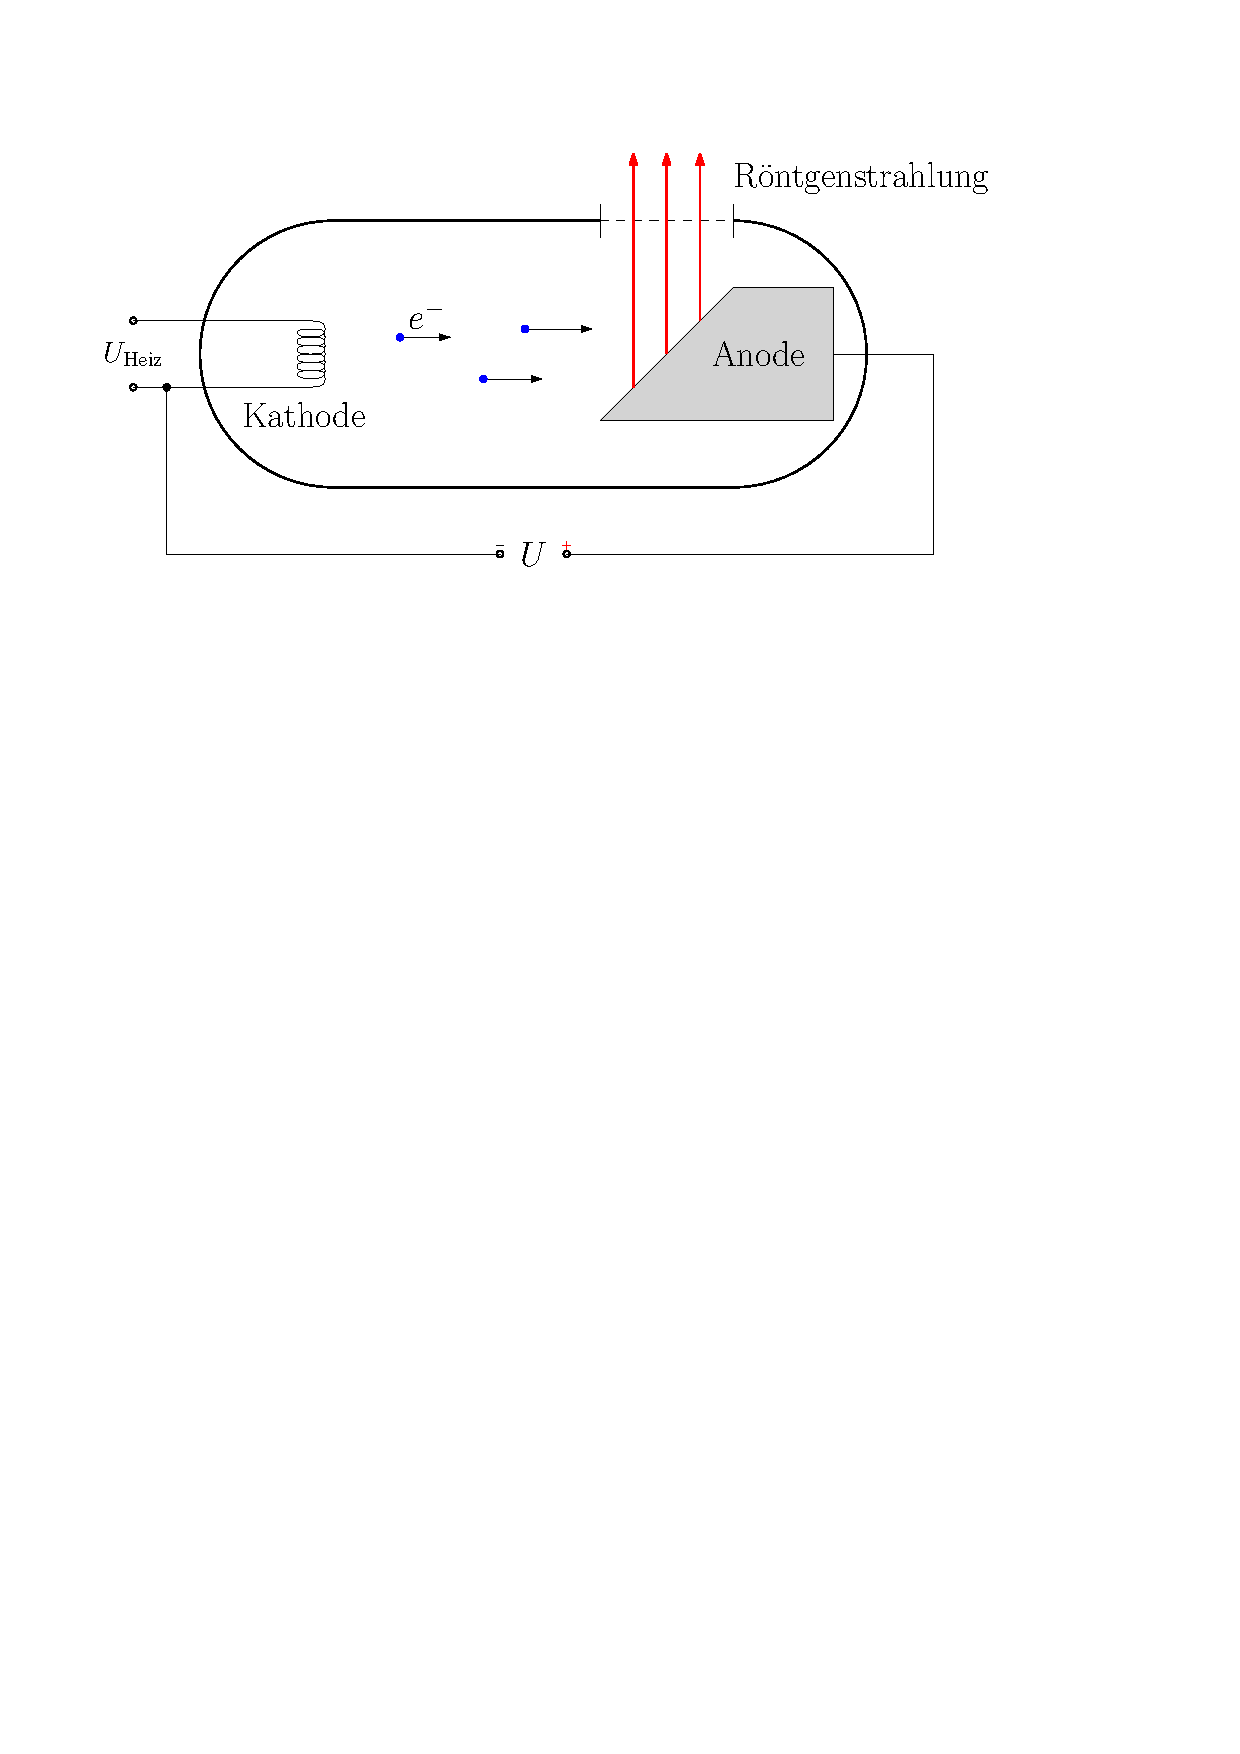
\includegraphics[width=0.75\textwidth]{./grafiken/roentgenroehre.pdf}
\caption{schematischer Aufbau einer Röntgenröhre}
\label{fig:roehre}
\end{figure}

\subsection{Röntgenfluoreszenz}
Als Röntgenfluoreszenz bezeichnet man die Entstehung sekundärer, fluoreszierender Röntgenstrahlung.
Dies geschieht ähnlich wie die Erzeugung charakteristischer Röntgenstrahlung, nur dass nun bereits erzeugte Röntgenstrahlung anstatt den energiereichen Elektronen zur Bestrahlung eines Elements verwendet werden.
Diese sekundäre Röntgenstrahlung weist wieder ein charakteristisches Spektrum auf, aus dem man auf das beschossene Element schließen kann.
Das Verfahren zur Elementbestimmung (oder Anteilen an Elementen in dem Target) nennt sich daher \textbf{Röntgenfluoreszenzanalyse}.

\subsection{Nachweis}
\label{sec:nachweis}
Zum Nachweis von Röntgenstrahlung werden in diesem Versuch Geiger-Müller-Zählrohre, Röntgenenergiedetektor und Röntgenfilm verwendet.

\subsubsection{Röntgenfilm}
Der Röntgenfilm ist mit einer speziellen Silberbromid Beschichtung ausgestattet, wobei aus \ce{Br-} Ionen und der einfallenden Röntgenstrahlung \ce{Br} und freie Elektronen entstehen.
Beim Entwickeln werden diese mit \ce{Ag+} zu Silberkörnern (\ce{Ag}) reduziert, was eine Schwarzfärbung des Films hervorruft.

\subsubsection{Geiger-Müller-Zählrohr}
Das Geiger-Müller-Zählrohr besteht aus einem Metallzylinder, der die Kathode darstellt und einem Draht im Inneren des Zylinders, der die Anode bildet.
Der Zylinder ist mit einem Gas unter hohem Druck gefüllt, wobei meistens Edelgas verwendet wird, da diese keinen negativen Ionen bilden, die den Betrieb stören können.
Bei Eintritt von Teilchen in das Zählrohr werden die Gasatome ionisiert und so freie Elektronen erzeugt.
Durch die zwischen Draht und Zylindermantel anliegende Spannung werden diese zum Draht beschleunigt.
Dadurch entsteht ein Stromimpuls, der dann an einem digitalen Zähler registriert wird, wobei die Anzahl Elektronen bei geladenen zu zählenden Teilchen und damit die Anzahl Impulse der Anzahl der einfallenden Teilchen entspricht.
Für den Betrieb ist die angelegte Gleichspannung zwischen Anode und Kathode entscheidend.
Bei zu geringer Spannung können die freien Elektronen auf der Beschleunigungstrecke wieder mit den Gasatomen rekombinieren (Rekombinationsbereich), wodurch die Messung verfälscht wird.
Erst ab einer bestimmten Gleichspannung erreichen alle Elektronen die Anode, womit dann die von der Strahlung im Zählrohr abgegebene Energie gemessen wird.
Beim Geiger-Müller-Zählrohr ist das Zählrohr so ausgelegt, dass die Elektronen durch die Beschleunigung Energien erreichen, die zur weiteren Ionisation der Gasatome führen, wodurch sich ein s.g. Lawineneffekt einstellt.

\begin{itemize}
  \item Aufbau
  \item Funktionsweise
  \item Totzeit
\end{itemize}

\subsubsection{Röntgenenergiedetektor}
\label{sec:energiedetektor}
\textbf{Aufbau:} PIN-Photodiode ($Q \propto E_\gamma$) -- Charge Amplifier (Integrator $U_\mathrm{out} \propto \int I = Q$) -- Verstärkerstufe ($U = V \cdot U_\mathrm{out}$)
Außerdem Kühlnug der PIN-Diode um den Leckstrom zu verringern (hier Peltier-Effekt)

\textbf{PIN-Photodiode:} Besteht aus einer PIN-Halbleiterschicht, wobei I für intrinischem Halbleiter (undotiert) steht.
Unter reverse Bias bildet sich eine Verarmungszone im intrinsischen Halbleiterbereich.
Wird ein Röntgenphoton in der intrinsischen Zone absorbiert (Photoeffekt) und löst ein Elektron aus den Halbleiteratomen, sodass ein Elektron-Loch Paar entsteht.
Das hochenergetische Elektron kann nun weitere Kristallatome ionisieren oder auch unter Ausstrahlung eines charakteristischen Röntgenphotons erneut ein Elektron-Loch Paar erzeugen.
Dies passiert sooft, bis die gesamte Energie des Röntgenphotons in Elektronen-Loch Paare umgewandelt wurde, deren Anzahl gegeben ist durch:
\begin{align}
  N = \frac{E_\gamma}{W_{e,\mathrm{Loch}}}
\end{align}
Dadurch entsteht ein Ladungsfluss proportional zur Energie des Röntgenquants.

\textbf{Funktionsweise:} Dieser Strom kann wird in einem Integrator (Op amp?) aufintegriert um die Gesamtladung zu erhalten.
Diese wird wiederum in einer nächsten Verstärkerstufe verstärkt, um eine zur Photonenenergie proportionale Spannung zu erhalten.

\textbf{Vielkanalanalysator:} Ein DAC die zur Photonenenergie proportionale (verstärkte) Spannung $U$ in einen digitalen Wert um, sodass aufgrund der endlichen Auflösung des DAC's die Energien in Bins (Histogram!) deren Breite durch das Auflösungsvermögen gegeben sind.
Mit jedem Impuls (Photondetektion) wird der zu dem digitalen Wert gehörende Bin um eins hochgezählt.

\textbf{Kalibrierung:} Aufgrund der unbekannten Proportionalitäten und Nullpunktsverschiebung muss die Energie anhand von zwei Kalibrationswerten
(Bestimmung von m und b) bestimmt werden.
\begin{align}
  E = m \cdot U_\mathrm{digital} + b
  \label{eq:kalibrierung}
\end{align}

Aus der Höhe der Linien im Count--Energie Diagramm kann der Massenanteil des jeweiligen Stoffes bestimmt werden, da die Höhe der Linie proportional zur Anzahl der strahlenden Atome ist.
Vergleicht man das aufgenommene Spektrum mit einem Referenzspektrum mit strahlenden Atomen:
\begin{align}
  n_0 = V \cdot \frac{\rho}{A}
\end{align}
($V$: durchstrahltes Volumen; $\rho$: Massendichte des Stoffes; $A$: Atomgewicht des Stoffes)
So kann die Höhe $H$ des Peaks im zu analysierenden Spektrum mit der im Referenzspektrum $H_0$ verglichen und daraus die Anzahl $n$ der Atome im zu analysierenden Spektrum berechnet werden:
\begin{align}
  n = n_0 \cdot \frac{H}{H_0}
\end{align}
Daher ergibt sich der Massenanteil des $i$-ten Referenzmaterials im zu analysierenden Spektrum zu:
\begin{align}
  C_i = \frac{n_i \cdot A_i}{\sum_j n_j \cdot A_j} = \frac{V \cdot \frac{\rho_i}{A_i} \cdot \frac{H_i}{H_{0,i}} \cdot A_i}{\sum_j V \cdot \frac{\rho_j}{A_j} \cdot \frac{H_j}{H_{0,j}}\cdot A_j} = \frac{\rho_i \cdot \frac{H_i}{H_{0,i}}}{\sum_j \rho_j \cdot \frac{H_j}{H_{0,j}}}
  \label{eq:masseanteile}
\end{align}
wobei das durchstrahlte Volumen der einzelnen Proben als gleich angenommen wird.

Was noch erwähnt werden sollte:
\begin{itemize}
  \item Elektron-Loch Bildung in pn-Grenzschichten
  \item Szintillationszähler
\end{itemize}

\subsection{Bragg-Reflexion}
Betrachtet man die Beugung von einfallender elektromagnetischer Strahlung an parallelen Netzebenen eines Einkristalls, so führt die Interferenz der gebeugten Wellen zu einer Ausbildung von Beugungsmaxima.
Bezeichnet $\beta$ den Winkel des einfallenden Strahls gegen die parallelen Netzebenen (Glanzwinkel), so erhält man konstruktive Interferenz, wenn der Weglängenunterschied zwischen zwei benachbarten Netzebenen ein ganzzahliges Vielfaches der Wellenlänge $\lambda$ ist:
\begin{align}
  \Delta s = m \lambda \quad \text{für } m \in \mathbb{N}
\end{align}
Dabei ist der Weglängenunterschied gegeben durch den Netzebenenabstand $d$ und dem Glanzwinkel $\beta$:
\begin{align}
  \Delta s = 2 d \sin(\beta)
\end{align}
und man erhält die \textbf{Bedingung für Bragg-Reflexion}:
\begin{align}
  2 d \sin(\beta) = m \lambda
  \label{eq:bragg}
\end{align}

\begin{figure}[h]
\centering
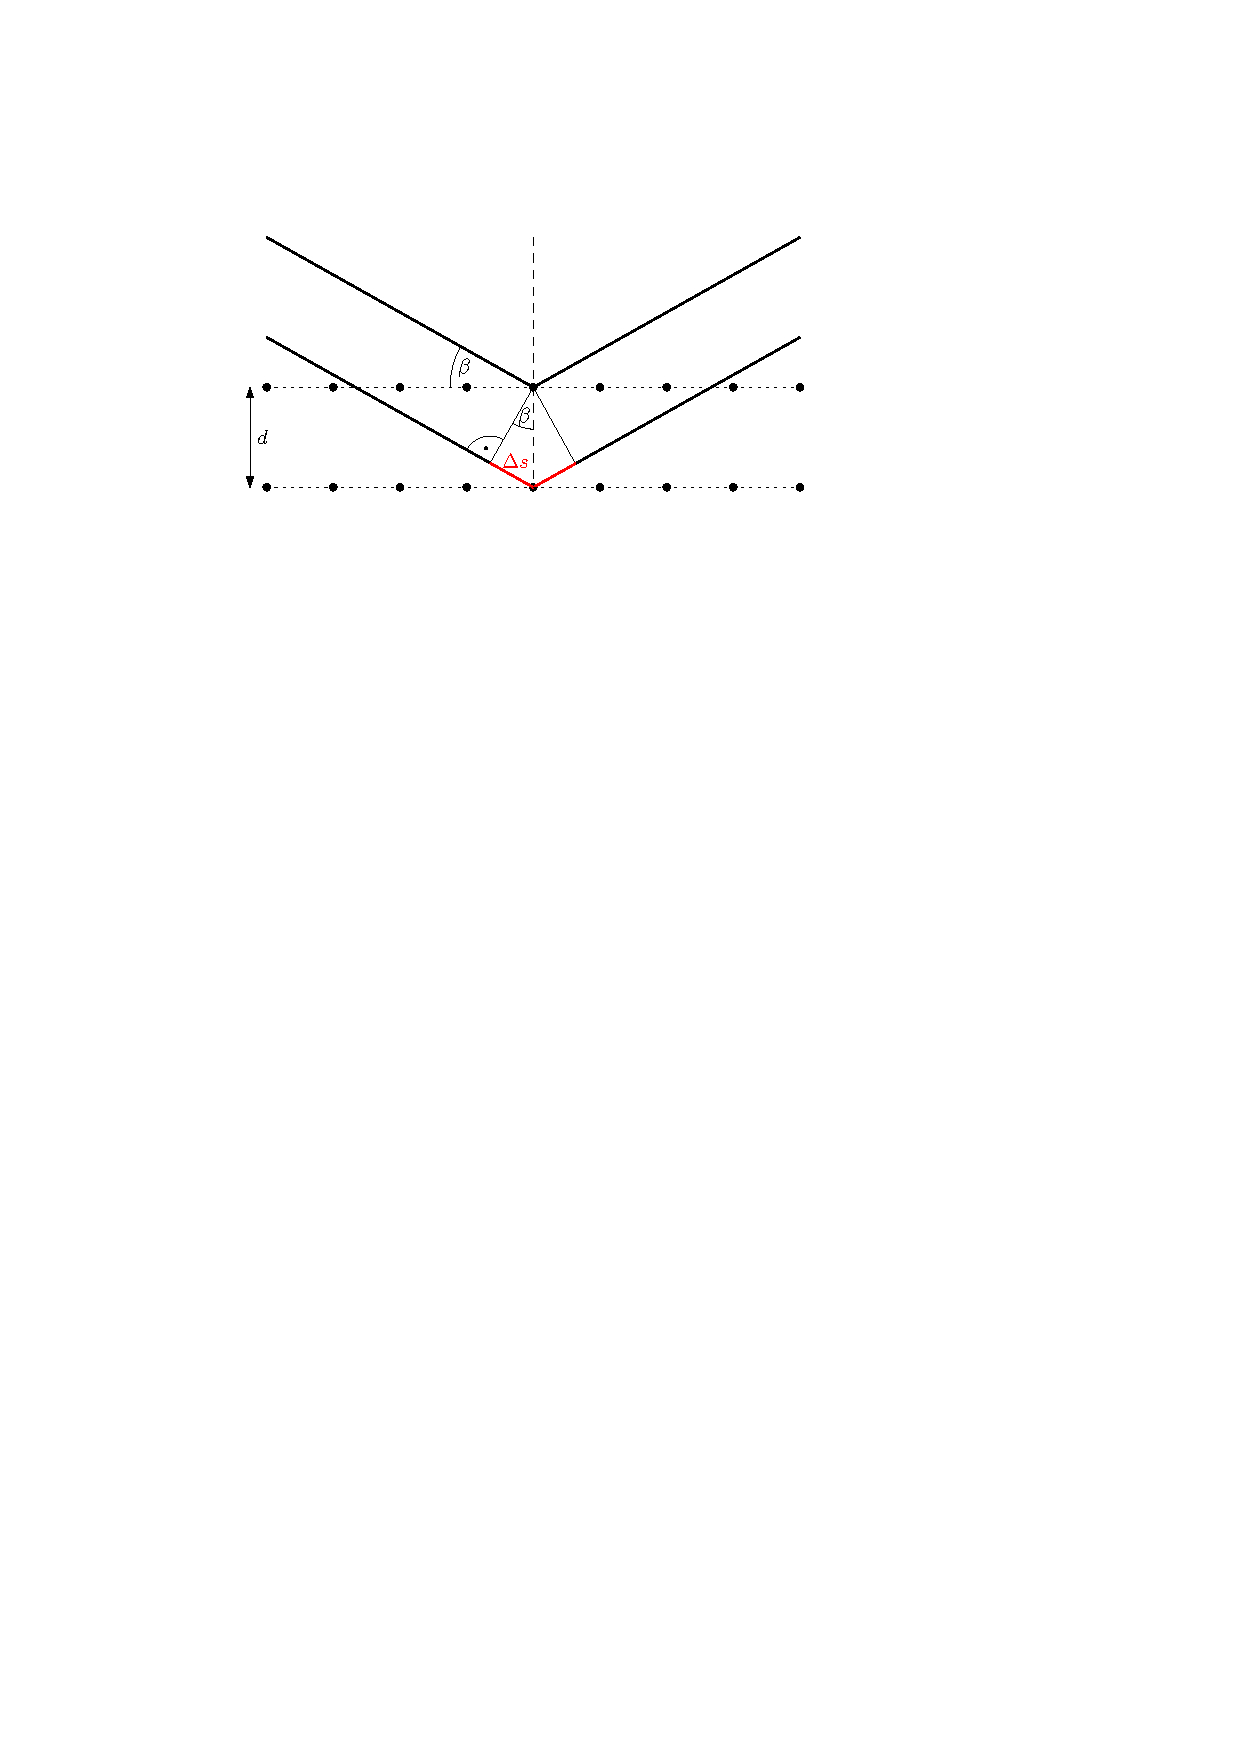
\includegraphics[width=0.75\textwidth]{./grafiken/bragg.pdf}
\caption{Zur Herleitung der Bragg-Bedingung}
\label{fig:bragg_bedingung}
\end{figure}

\begin{itemize}
  \item Röntgenbeugung (muss noch erklärt werden)
\end{itemize}

\subsection{Laue-Verfahren}

\subsubsection{Elementarzelle}
Translationsvektoren mit Basis $(\vec{a}, \vec{b}, \vec{c})$

\subsubsection{Millersche Indizes}

Zur Beschreibung von Gitterebenen in einem Kristall nutzt man die s.g. Millerschen Indizes $(hkl)$, mit denen eine Gitterebene eindeutig beschrieben ist.
Man legt dabei das reale Gitter im Kristall mit den Einheitsvektoren $\vec{a}$, $\vec{b}$, $\vec{c}$ zugrunde und betrachtet die Schnittpunkte der betrachteten Gitterebene mit den jeweiligen Achsen.
Die Schnittpunkte werden dann geschrieben als S$_i=m_i\vec{e}_i$ mit $i=1,2,3$ und $\vec{e}_i= \vec{a}, \vec{b}, \vec{c}$.
Die Millerschen Indizes erhält man, wenn man die Kehrwerte $\frac{1}{m_i}$ betrachtet und $p$ so wählt, dass die reziproken Werte ganze, teilerfremde Zahlen werden\cite{demtroeder}:
\begin{align}
h=\dfrac{p}{m_1} \quad\quad k=\dfrac{p}{m_2} \quad\quad l=\dfrac{p}{m_3}
\end{align}
Betrachte dazu auch das Beispiel in Abbildung \ref{fig:millerindizes}.
\begin{figure}[h]
\centering
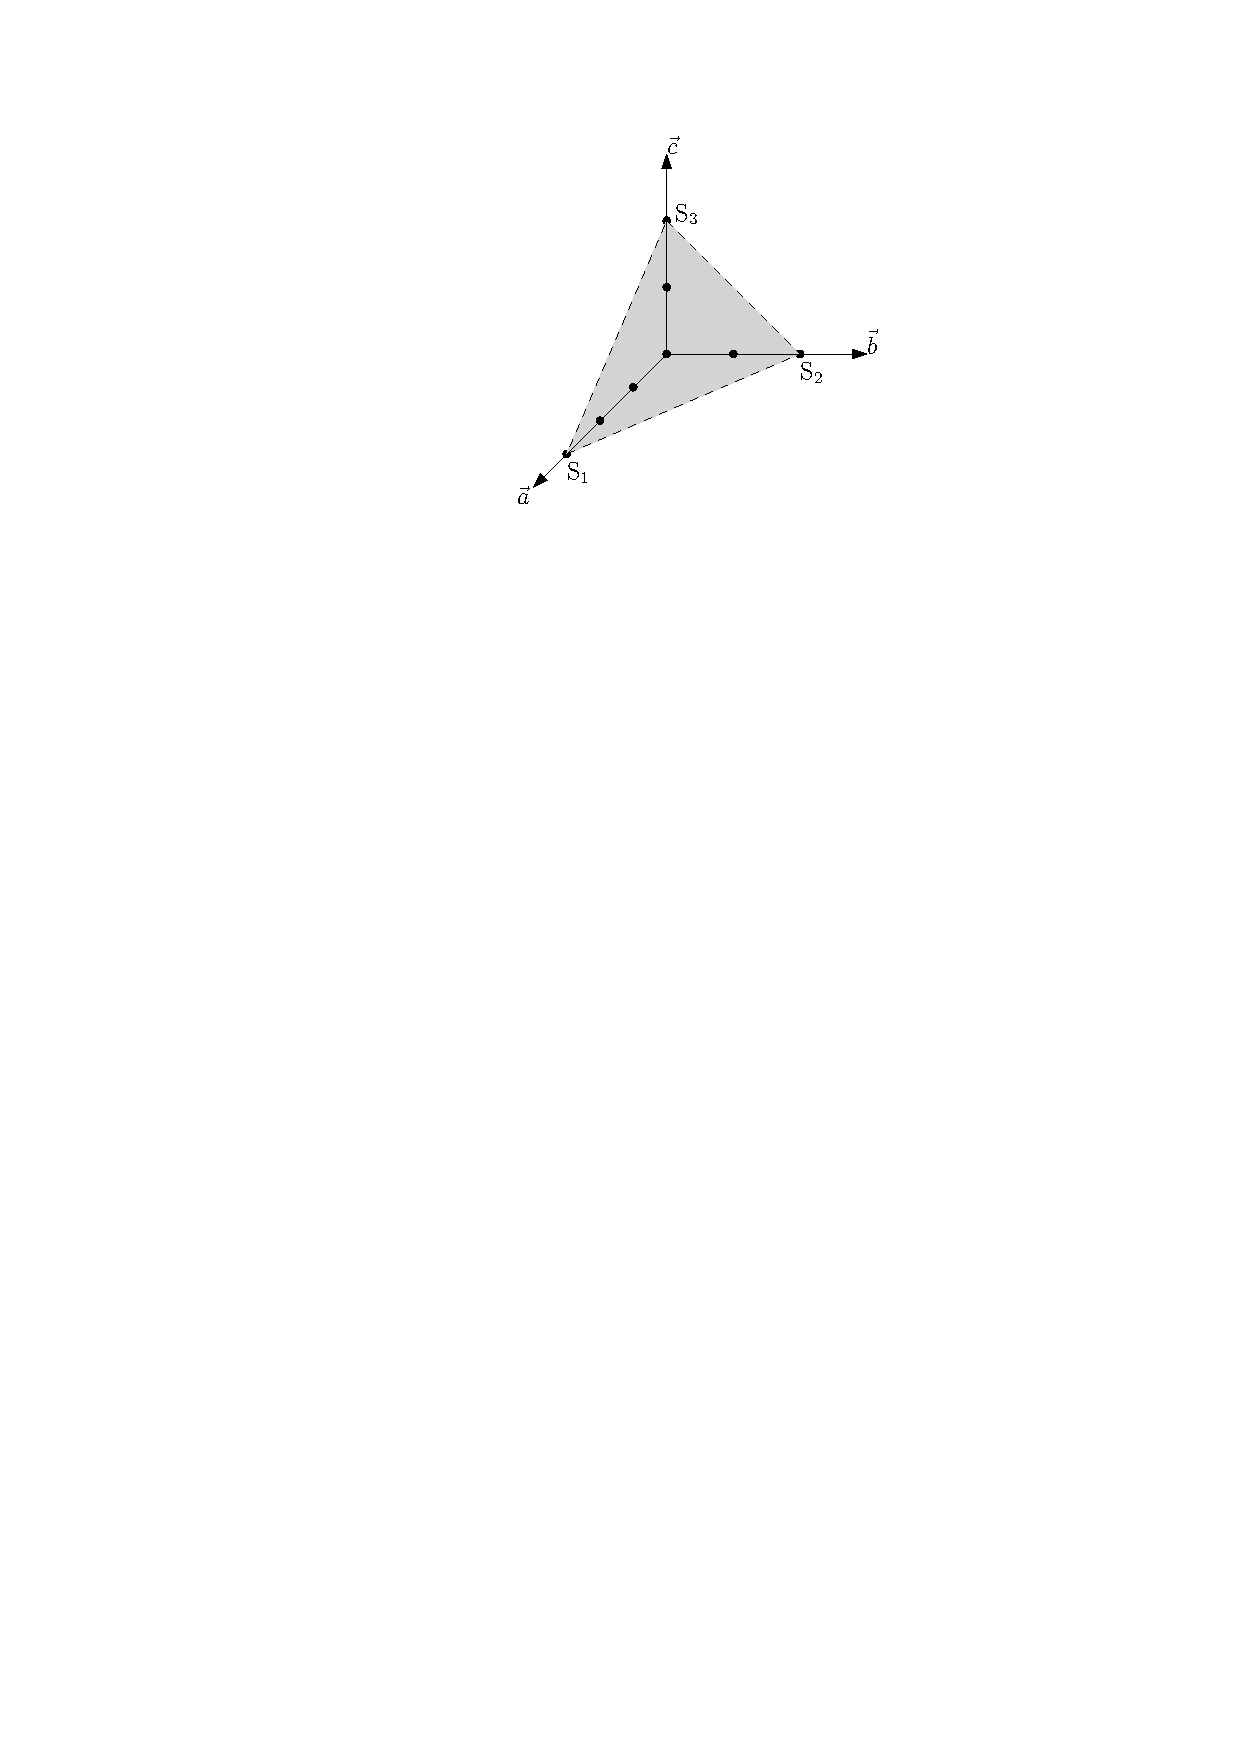
\includegraphics[width=0.4\textwidth]{./grafiken/millerindizes.pdf}
\caption{Beispiel zur Bestimmung der Millerindizes mit $m_1=3$, $m_2=2$, $m_3=2$. Die Ebene wird dann beschrieben durch $(233)$ (mit $p=6$).}
\label{fig:millerindizes}
\end{figure}

\subsubsection{reziprokes Gitter}
Definiert anhand der Basisvektoren des Gitters (demtröder):

\begin{align}
  \vec{a}^{*} = \frac{2\pi}{V_\mathrm{E}} \cdot ( \vec{b} \times \vec{c} ) \nonumber\\
  \vec{b}^{*} = \frac{2\pi}{V_\mathrm{E}} \cdot ( \vec{c} \times \vec{a} ) \nonumber\\
  \vec{c}^{*} = \frac{2\pi}{V_\mathrm{E}} \cdot ( \vec{a} \times \vec{b} )
\end{align}
Mit dem Volumen der Elementarzelle
\begin{align}
  V_\mathrm{E} = \vec{a} \cdot \left( b \times c \right)
\end{align}
Besondere Zusammenhänge mit den durch die millersche Indizes $(hkl)$ ausgezeichnete Ebenenschar:
\begin{align}
  \vec{G} = h \vec{a}^{*} + k \vec{b}^{*} + l \vec{c}^{*}
\end{align}
steht senkrecht auf der Ebenenschar $(hkl)$.
\begin{align}
  | \vec{G} | = \frac{2\pi}{d_{hkl}}
  \label{eq:netzebenenabstand}
\end{align}
wobei $d_{hkl}$ der Abstand zweier benachbarter Ebenen ist.



\begin{itemize}
  \item Laue--Bedingung
  \item reziprokes Gitter
  \item Elementarzelle
  \item Glanzwinkel
  \item Netzebenenabstand
\end{itemize}

\section{Versuchsteil 1: Bragg-Reflekion}
Im Folgenden wollen wir unter Ausnutzung von Bragg-Reflektion an einem NaCl-Einkristall die Wellenlänge und Energie des charakteristischen Röntgenspektrums einer unbekannten Röhrenanode bestimmen und anhand dessen das Anodenmaterial bestimmen.
Anschließend wird die Feinstrukturaufspaltung $\Delta \lambda$ der $K_\alpha$-Linie der charakteristischen Röntgenstrahlung einer Molybdän-Anode in vierter Beugungsordnung bestimmt.

\subsection{Versuchsdurchführung}
\subsubsection{Bestimmung der charakteristischen Röntgenstrahlung einer unbekannten Röhre}
\begin{figure}[h]
\centering
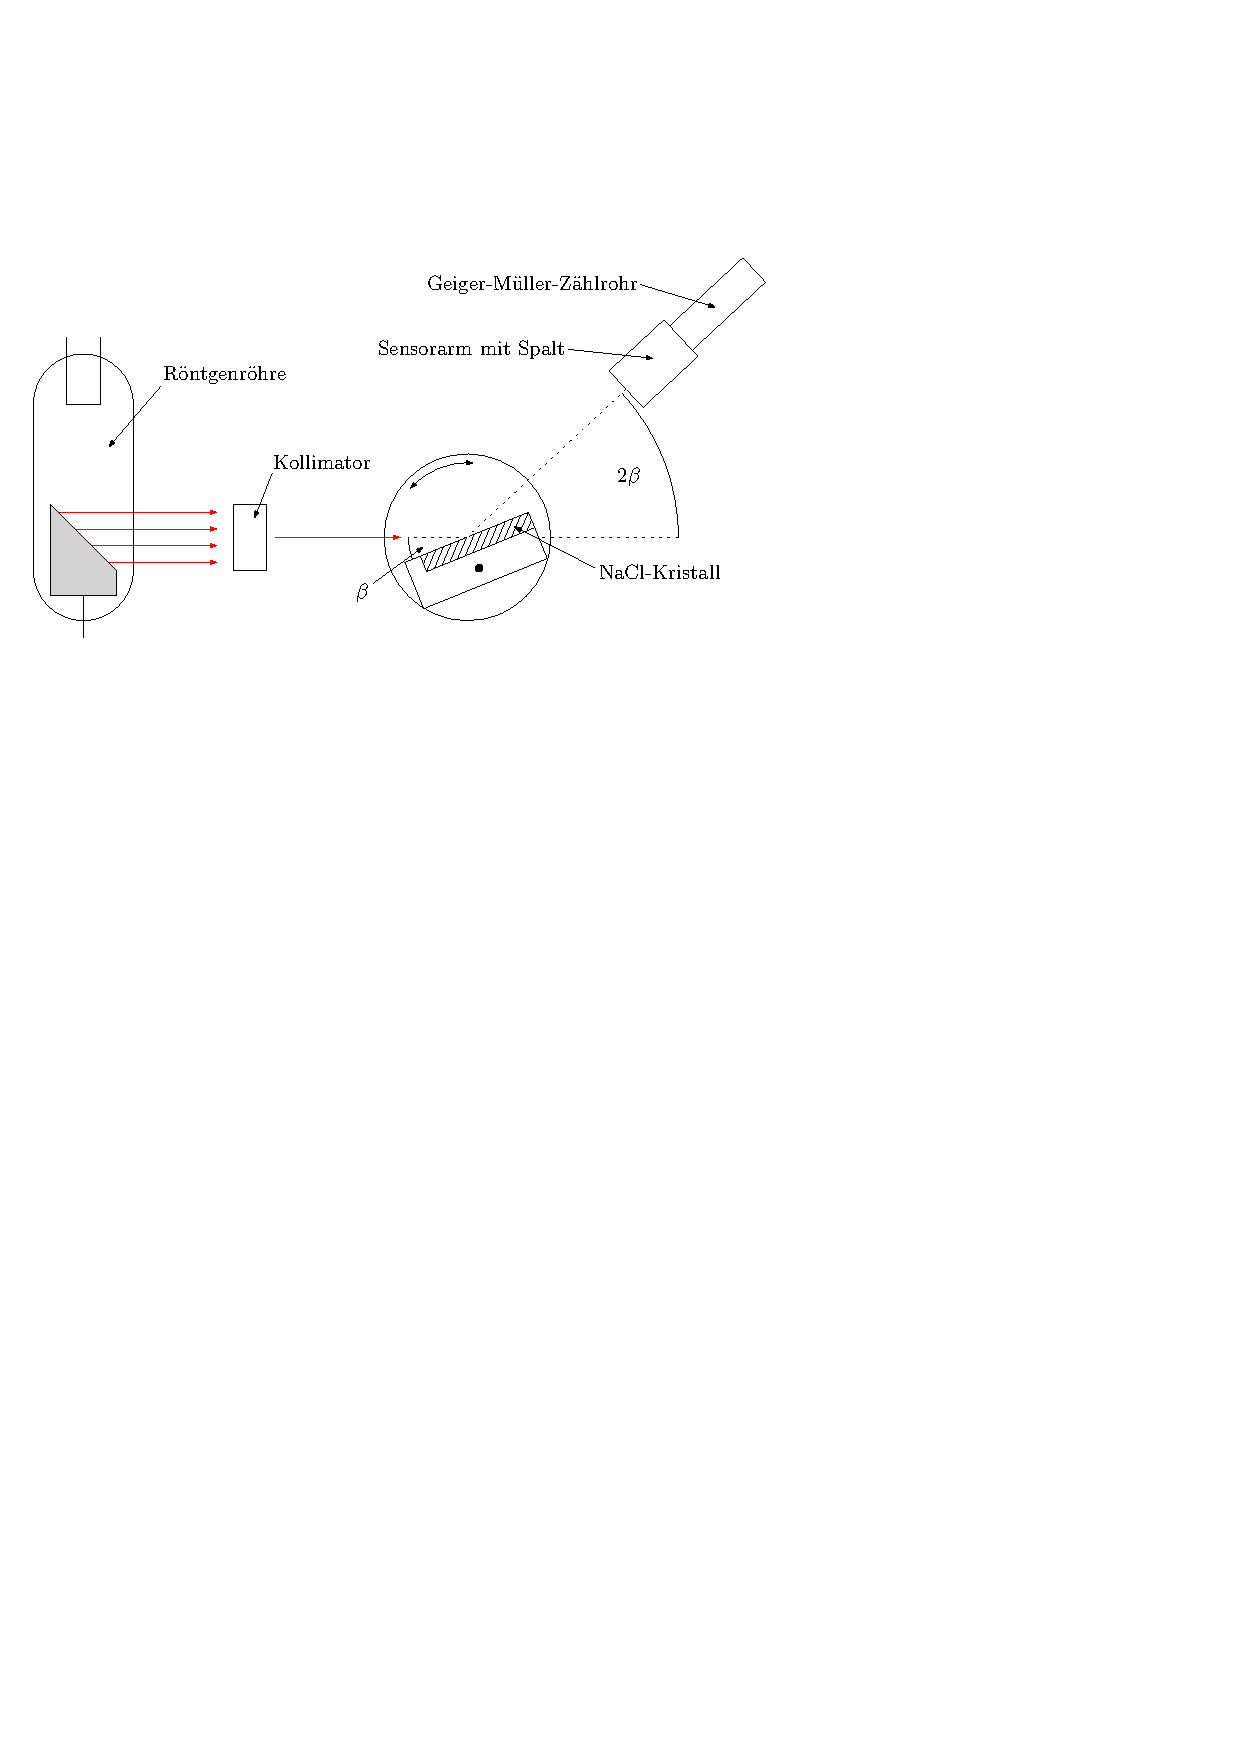
\includegraphics[width=0.9\textwidth]{./grafiken/aufbau_bragg.pdf}
\caption{Versuchsaufbau zur Bragg-Reflektion am NaCl-Kristall}
\label{fig:bragg_aufbau}
\end{figure}
Zur Aufnahme des charakteristischen Röntgenspektrums einer unbekannten Anode wird das Vollschutzröntgengerät verwendet, dessen innerer Aufbau in Abbildung \ref{fig:bragg_aufbau} dargestellt ist.
Zunächst tauschen wir die installierte Röntgenröhre gegen die \textbf{unbekannte Röntgenröhre 3} aus.
Zur Kollimation der Röntgenstrahlung der Röntgenröhre verwenden wir den Kollimatorspalt der Breite \SI{1}{\milli\metre}, welcher in den vorgesehenen Sockel des Vollschutzröntgengeräts eingesetzt wird.
Dies ist nötig, da die Röntgenstrahlung nicht parallel aus der Röntgenröhre austritt und daher ohne Kollimation kein scharfes Spektrum entsteht, da die Strahlen unter verschiedenen Glanzwinkeln auf das Target treffen.

Im Experimentierraum des Röntgengeräts befindet sich das Goniometer, an welchem zunächst der Sensorarm mit \SI{1}{\milli\metre} Spalt befestigt wird.
In diesen setzen wir das Geiger-Müller-Zählrohr ein, (anschließen an die Elektronik).
Schließlich wird der Targettisch an dem Goniometer befestigt und der NaCl-Kristall so auf dem Tisch befestigt, dass dessen Rotationsachse etwa auf der Kristalloberfläche liegt.
Dabei wurden Sensorarm und Goniometer so positioniert, dass der Abstand Kollimatorspalt--Target und Sensorarm--Target \num{5} bis \SI{6}{\centi\metre} beträgt.
Das Goniometer dient nun zur computergesteuerten Einstellung der Winkel von Targettisch $\beta_\mathrm{Target}$ und Sensorarm $\beta_\mathrm{Sensor}$ zur Horizontalen.
Da bei Bragg-Reflektion der Winkel des einfallenden Strahls zum Target gleich dem des Ausfallenden ist, wird das Goniometer im \emph{Coupled}-Modus betrieben, welcher das Target und den Sensorarm stets so einstellt, dass die Bedingung $\beta = \beta_\mathrm{Target} = 2\beta_\mathrm{Sensor}$ erfüllt ist.

Die eigentliche Messung wird nun computergesteuert durchgeführt.
Dabei verwenden wir eine Röhrenspannung von \SI{35}{\kilo\volt} mit einem Emissionsstrom zwischen Glühkathode und Anode von \SI{1}{\milli\ampere}.
Wir vermessen einen Glanzwinkelbereich von $\beta_\mathrm{min} = \SI{2,0}{\degree}$ bis $\beta_\mathrm{max} = \SI{25,0}{\degree}$ in Schritten von $\Delta \beta = \SI{0,1}{\degree}$, wobei jede Winkeleinstellung für $\Delta t = \SI{10}{\second}$ gehalten wird und die mittlere Zählrate des Zählrohrs über dem Zeitintervall durch das Programm gemessen wird.

Nach dem Abschluss der Messung wurde das Spektrum mithilfe der Funktion \emph{'Peakschwerpunkt berechnen'} des Programmes ausgemessen. Auf die genaue Vorgehensweise wird dabei in der Auswertung eingegangen.

\subsubsection{Bestimmung der Feinstruktur der $K_\alpha$-Linie von Molybdän}
Die Feinstrukturaufspaltung $\Delta \lambda$ der $K_\alpha$-Linie von Molybdän ist sehr klein; um diese dennoch aufzulösen, kann eine höhere Beugungsordnungen vermessen werden.
Dies sieht man leicht, wenn man die Bragg-Bedingung nach dem Glanzwinkel umstellt:
\begin{align}
  \beta = \arcsin \left( \frac{m \lambda}{2 d} \right)
\end{align}
und das Differential bildet:
\begin{align}
  \mathrm{d}\beta = \frac{\partial \beta}{\partial \lambda} \mathrm{d}\lambda = \frac{m\, \mathrm{d}\lambda}{\sqrt{4 d^2 - m^2 \lambda^2}}
\end{align}
Betrachtet man dies als lineare Näherung, so ist die Glanzwinkeldifferenz $\Delta \beta$ der Feinstrukturaufspaltung $\Delta \lambda$ eine in $m$ monoton steigende Funktion für $m < \frac{2d}{\lambda}$.
Wir erhalten also eine größere Winkeldifferenz in höheren Ordnungen, sodass wir in der Lage sind die $K_\alpha$-Linie von Molybdän in vierter Ordnung aufzulösen.

Der Versuchsaufbau entspricht zu großen Teilen dem des vorigen Versuchsteil.
Die Unterschiede bestehen in der nun verwendeten Molybdän-Röhre, sowie dem Austausch des Kollimators sowie des Zählrohrspalts durch hochauflösende \SI{0,3}{\milli\metre} Spalte, um ein hohes Winkelauflösungsvermögen zu erreichen.
Darüberhinaus wurde die automatische Kristallkalibration der Software verwendet um die Nullstellung des Goniometers einzustellen.

Dem Intensitätsverlust aufgrund der Verwendung dünnerer Spalte wird entgegengewirkt, indem die Messzeit pro Winkelschritt auf $\Delta t = \SI{120}{\second}$ erhöht wird.
Wir vermessen einen Glanzwinkelbereich von $\beta_\mathrm{min} = \SI{28,50}{\degree}$ bis $\beta_\mathrm{max} = \SI{32,00}{\degree}$ in Schritten $\Delta \beta = \SI{0,01}{\degree}$ über Nacht.

Am Folgetag wurden auch hier mithilfe von \emph{Cassy Lab} die Peakschwerpunkte der Feinstruktur bestimmt (näheres in der Auswertung).

% Temporär damit ich nicht wahnsinnig werde
\newpage
\subsection{Messdaten}
\subsubsection{Charakteristischen Röntgenstrahlung einer unbekannten Röhre}


\begin{figure}[!h]
\centering
% GNUPLOT: LaTeX picture with Postscript
\begingroup
  \makeatletter
  \providecommand\color[2][]{%
    \GenericError{(gnuplot) \space\space\space\@spaces}{%
      Package color not loaded in conjunction with
      terminal option `colourtext'%
    }{See the gnuplot documentation for explanation.%
    }{Either use 'blacktext' in gnuplot or load the package
      color.sty in LaTeX.}%
    \renewcommand\color[2][]{}%
  }%
  \providecommand\includegraphics[2][]{%
    \GenericError{(gnuplot) \space\space\space\@spaces}{%
      Package graphicx or graphics not loaded%
    }{See the gnuplot documentation for explanation.%
    }{The gnuplot epslatex terminal needs graphicx.sty or graphics.sty.}%
    \renewcommand\includegraphics[2][]{}%
  }%
  \providecommand\rotatebox[2]{#2}%
  \@ifundefined{ifGPcolor}{%
    \newif\ifGPcolor
    \GPcolortrue
  }{}%
  \@ifundefined{ifGPblacktext}{%
    \newif\ifGPblacktext
    \GPblacktexttrue
  }{}%
  % define a \g@addto@macro without @ in the name:
  \let\gplgaddtomacro\g@addto@macro
  % define empty templates for all commands taking text:
  \gdef\gplbacktext{}%
  \gdef\gplfronttext{}%
  \makeatother
  \ifGPblacktext
    % no textcolor at all
    \def\colorrgb#1{}%
    \def\colorgray#1{}%
  \else
    % gray or color?
    \ifGPcolor
      \def\colorrgb#1{\color[rgb]{#1}}%
      \def\colorgray#1{\color[gray]{#1}}%
      \expandafter\def\csname LTw\endcsname{\color{white}}%
      \expandafter\def\csname LTb\endcsname{\color{black}}%
      \expandafter\def\csname LTa\endcsname{\color{black}}%
      \expandafter\def\csname LT0\endcsname{\color[rgb]{1,0,0}}%
      \expandafter\def\csname LT1\endcsname{\color[rgb]{0,1,0}}%
      \expandafter\def\csname LT2\endcsname{\color[rgb]{0,0,1}}%
      \expandafter\def\csname LT3\endcsname{\color[rgb]{1,0,1}}%
      \expandafter\def\csname LT4\endcsname{\color[rgb]{0,1,1}}%
      \expandafter\def\csname LT5\endcsname{\color[rgb]{1,1,0}}%
      \expandafter\def\csname LT6\endcsname{\color[rgb]{0,0,0}}%
      \expandafter\def\csname LT7\endcsname{\color[rgb]{1,0.3,0}}%
      \expandafter\def\csname LT8\endcsname{\color[rgb]{0.5,0.5,0.5}}%
    \else
      % gray
      \def\colorrgb#1{\color{black}}%
      \def\colorgray#1{\color[gray]{#1}}%
      \expandafter\def\csname LTw\endcsname{\color{white}}%
      \expandafter\def\csname LTb\endcsname{\color{black}}%
      \expandafter\def\csname LTa\endcsname{\color{black}}%
      \expandafter\def\csname LT0\endcsname{\color{black}}%
      \expandafter\def\csname LT1\endcsname{\color{black}}%
      \expandafter\def\csname LT2\endcsname{\color{black}}%
      \expandafter\def\csname LT3\endcsname{\color{black}}%
      \expandafter\def\csname LT4\endcsname{\color{black}}%
      \expandafter\def\csname LT5\endcsname{\color{black}}%
      \expandafter\def\csname LT6\endcsname{\color{black}}%
      \expandafter\def\csname LT7\endcsname{\color{black}}%
      \expandafter\def\csname LT8\endcsname{\color{black}}%
    \fi
  \fi
  \setlength{\unitlength}{0.0500bp}%
  \begin{picture}(7200.00,4320.00)%
    \gplgaddtomacro\gplbacktext{%
      \csname LTb\endcsname%
      \put(1078,704){\makebox(0,0)[r]{\strut{} 0}}%
      \csname LTb\endcsname%
      \put(1078,1295){\makebox(0,0)[r]{\strut{} 500}}%
      \csname LTb\endcsname%
      \put(1078,1886){\makebox(0,0)[r]{\strut{} 1000}}%
      \csname LTb\endcsname%
      \put(1078,2477){\makebox(0,0)[r]{\strut{} 1500}}%
      \csname LTb\endcsname%
      \put(1078,3068){\makebox(0,0)[r]{\strut{} 2000}}%
      \csname LTb\endcsname%
      \put(1078,3659){\makebox(0,0)[r]{\strut{} 2500}}%
      \csname LTb\endcsname%
      \put(1210,484){\makebox(0,0){\strut{} 0}}%
      \csname LTb\endcsname%
      \put(2329,484){\makebox(0,0){\strut{} 5}}%
      \csname LTb\endcsname%
      \put(3447,484){\makebox(0,0){\strut{} 10}}%
      \csname LTb\endcsname%
      \put(4566,484){\makebox(0,0){\strut{} 15}}%
      \csname LTb\endcsname%
      \put(5684,484){\makebox(0,0){\strut{} 20}}%
      \csname LTb\endcsname%
      \put(6803,484){\makebox(0,0){\strut{} 25}}%
      \put(176,2181){\rotatebox{-270}{\makebox(0,0){\strut{}Z\"ahlrate}}}%
      \put(4006,154){\makebox(0,0){\strut{}Glanzwinkel $\theta$ / \si{\degree}}}%
      \put(4006,3989){\makebox(0,0){\strut{}Gemessene Z\"ahlrate für unterschiedliche Winkel bei Bragg-Beugung}}%
    }%
    \gplgaddtomacro\gplfronttext{%
      \csname LTb\endcsname%
      \put(5816,3486){\makebox(0,0)[r]{\strut{}Zählrate}}%
    }%
    \gplbacktext
    \put(0,0){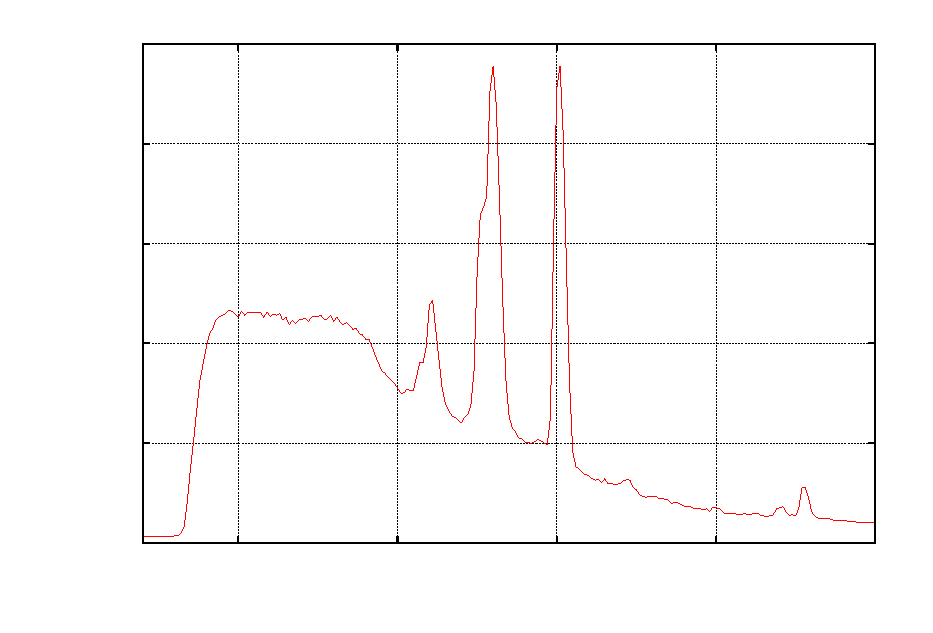
\includegraphics{./plots/anode3}}%
    \gplfronttext
  \end{picture}%
\endgroup

\caption{Aufgenommenes Röntgenspektrum der unbekannten Anode bei Bragg-Streuung an einem NaCl-Kristall}
\label{fig:anode3}
\end{figure}

\begin{table}[!h]
\centering
\begin{tabular}{lSScSS}
\toprule
{Peaknummer} & {Winkel $\beta / \si{\degree}$} & {Fehler $\Delta\beta / \si{\degree}$} & Ordnung & {Energie $E / \si{\electronvolt}$} & {Fehler $\Delta E / \si{\electronvolt}$}\\
\midrule
1&	11.047&	0.213&	1	&	11495.6&	218.9 \\
2&	12.919&	0.259&	1	&	9852.3&	194.2\\
3&	15.108&	0.148&	1	&	8451.2&	80.9\\
4&	17.242&	0.135&		&	7431.4&	56.4\\
5&	20.023&	0.101&		&	6433.2&	31.1\\
6&	22.037&	0.099&	2	&	5870.7&	25.1\\
7&	22.780&	0.104&	2	&	5688.9&	24.6\\
\bottomrule
\end{tabular}
\caption{Peakschwerpunkte in der Grobstruktur der unbekannten Anode und Umrechnung in die entsprechende Energie}
\label{tab:peakschwerpunkt_grobstruktur}
\end{table}

\newpage
\subsubsection{Feinstruktur der $K_\alpha$-Linie von Molybdän}

\begin{figure}[!h]
\centering
% GNUPLOT: LaTeX picture with Postscript
\begingroup
  \makeatletter
  \providecommand\color[2][]{%
    \GenericError{(gnuplot) \space\space\space\@spaces}{%
      Package color not loaded in conjunction with
      terminal option `colourtext'%
    }{See the gnuplot documentation for explanation.%
    }{Either use 'blacktext' in gnuplot or load the package
      color.sty in LaTeX.}%
    \renewcommand\color[2][]{}%
  }%
  \providecommand\includegraphics[2][]{%
    \GenericError{(gnuplot) \space\space\space\@spaces}{%
      Package graphicx or graphics not loaded%
    }{See the gnuplot documentation for explanation.%
    }{The gnuplot epslatex terminal needs graphicx.sty or graphics.sty.}%
    \renewcommand\includegraphics[2][]{}%
  }%
  \providecommand\rotatebox[2]{#2}%
  \@ifundefined{ifGPcolor}{%
    \newif\ifGPcolor
    \GPcolortrue
  }{}%
  \@ifundefined{ifGPblacktext}{%
    \newif\ifGPblacktext
    \GPblacktexttrue
  }{}%
  % define a \g@addto@macro without @ in the name:
  \let\gplgaddtomacro\g@addto@macro
  % define empty templates for all commands taking text:
  \gdef\gplbacktext{}%
  \gdef\gplfronttext{}%
  \makeatother
  \ifGPblacktext
    % no textcolor at all
    \def\colorrgb#1{}%
    \def\colorgray#1{}%
  \else
    % gray or color?
    \ifGPcolor
      \def\colorrgb#1{\color[rgb]{#1}}%
      \def\colorgray#1{\color[gray]{#1}}%
      \expandafter\def\csname LTw\endcsname{\color{white}}%
      \expandafter\def\csname LTb\endcsname{\color{black}}%
      \expandafter\def\csname LTa\endcsname{\color{black}}%
      \expandafter\def\csname LT0\endcsname{\color[rgb]{1,0,0}}%
      \expandafter\def\csname LT1\endcsname{\color[rgb]{0,1,0}}%
      \expandafter\def\csname LT2\endcsname{\color[rgb]{0,0,1}}%
      \expandafter\def\csname LT3\endcsname{\color[rgb]{1,0,1}}%
      \expandafter\def\csname LT4\endcsname{\color[rgb]{0,1,1}}%
      \expandafter\def\csname LT5\endcsname{\color[rgb]{1,1,0}}%
      \expandafter\def\csname LT6\endcsname{\color[rgb]{0,0,0}}%
      \expandafter\def\csname LT7\endcsname{\color[rgb]{1,0.3,0}}%
      \expandafter\def\csname LT8\endcsname{\color[rgb]{0.5,0.5,0.5}}%
    \else
      % gray
      \def\colorrgb#1{\color{black}}%
      \def\colorgray#1{\color[gray]{#1}}%
      \expandafter\def\csname LTw\endcsname{\color{white}}%
      \expandafter\def\csname LTb\endcsname{\color{black}}%
      \expandafter\def\csname LTa\endcsname{\color{black}}%
      \expandafter\def\csname LT0\endcsname{\color{black}}%
      \expandafter\def\csname LT1\endcsname{\color{black}}%
      \expandafter\def\csname LT2\endcsname{\color{black}}%
      \expandafter\def\csname LT3\endcsname{\color{black}}%
      \expandafter\def\csname LT4\endcsname{\color{black}}%
      \expandafter\def\csname LT5\endcsname{\color{black}}%
      \expandafter\def\csname LT6\endcsname{\color{black}}%
      \expandafter\def\csname LT7\endcsname{\color{black}}%
      \expandafter\def\csname LT8\endcsname{\color{black}}%
    \fi
  \fi
  \setlength{\unitlength}{0.0500bp}%
  \begin{picture}(7200.00,4320.00)%
    \gplgaddtomacro\gplbacktext{%
      \csname LTb\endcsname%
      \put(682,704){\makebox(0,0)[r]{\strut{} 1}}%
      \csname LTb\endcsname%
      \put(682,1126){\makebox(0,0)[r]{\strut{} 2}}%
      \csname LTb\endcsname%
      \put(682,1548){\makebox(0,0)[r]{\strut{} 3}}%
      \csname LTb\endcsname%
      \put(682,1970){\makebox(0,0)[r]{\strut{} 4}}%
      \csname LTb\endcsname%
      \put(682,2393){\makebox(0,0)[r]{\strut{} 5}}%
      \csname LTb\endcsname%
      \put(682,2815){\makebox(0,0)[r]{\strut{} 6}}%
      \csname LTb\endcsname%
      \put(682,3237){\makebox(0,0)[r]{\strut{} 7}}%
      \csname LTb\endcsname%
      \put(682,3659){\makebox(0,0)[r]{\strut{} 8}}%
      \csname LTb\endcsname%
      \put(814,484){\makebox(0,0){\strut{} 28}}%
      \csname LTb\endcsname%
      \put(1479,484){\makebox(0,0){\strut{} 28.5}}%
      \csname LTb\endcsname%
      \put(2145,484){\makebox(0,0){\strut{} 29}}%
      \csname LTb\endcsname%
      \put(2810,484){\makebox(0,0){\strut{} 29.5}}%
      \csname LTb\endcsname%
      \put(3476,484){\makebox(0,0){\strut{} 30}}%
      \csname LTb\endcsname%
      \put(4141,484){\makebox(0,0){\strut{} 30.5}}%
      \csname LTb\endcsname%
      \put(4807,484){\makebox(0,0){\strut{} 31}}%
      \csname LTb\endcsname%
      \put(5472,484){\makebox(0,0){\strut{} 31.5}}%
      \csname LTb\endcsname%
      \put(6138,484){\makebox(0,0){\strut{} 32}}%
      \csname LTb\endcsname%
      \put(6803,484){\makebox(0,0){\strut{} 32.5}}%
      \put(176,2181){\rotatebox{-270}{\makebox(0,0){\strut{}Z\"ahlrate / \si{\per\second}}}}%
      \put(3808,154){\makebox(0,0){\strut{}Glanzwinkel $\beta$ / \si{\degree}}}%
      \put(3808,3989){\makebox(0,0){\strut{}Gemessene Z\"ahlrate für unterschiedliche Winkel bei Bragg-Beugung (Feinstrukturaufspaltung)}}%
      \put(3749,3511){\makebox(0,0)[l]{\strut{}1}}%
      \put(3988,2507){\makebox(0,0)[l]{\strut{}2}}%
    }%
    \gplgaddtomacro\gplfronttext{%
    }%
    \gplbacktext
    \put(0,0){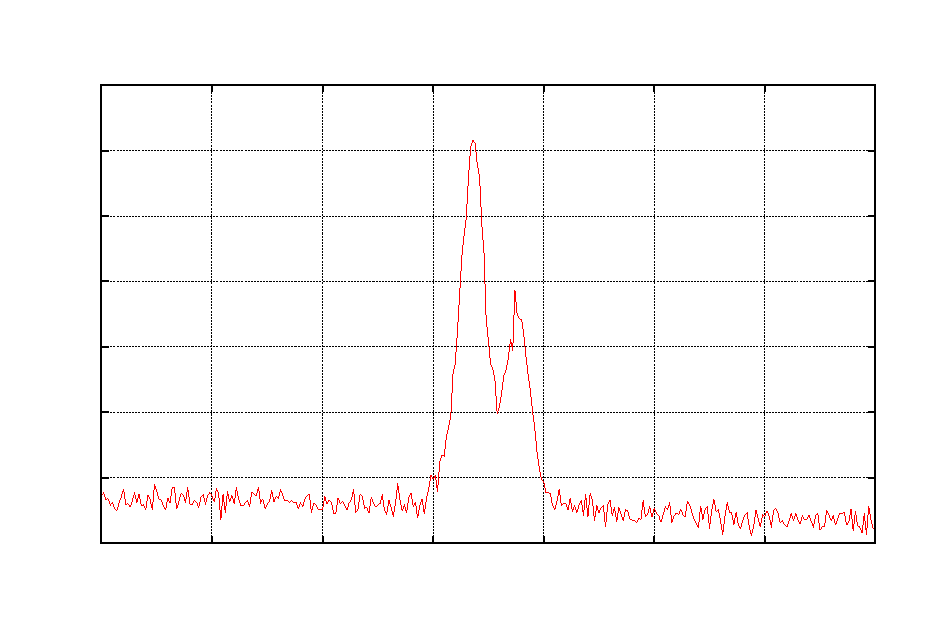
\includegraphics{./plots/feinstruktur}}%
    \gplfronttext
  \end{picture}%
\endgroup

\caption{Feinstrukturaufspaltung im Röntgenspektrum der Molybdänanode bei Bragg-Streuung (in vierter Ordnung) an einem NaCl-Kristall}
\label{fig:feinstruktur}
\end{figure}

\begin{table}[!h]
\centering
\begin{tabular}{lSS}
\toprule
{\#} & {$\beta_\mathrm{Peak} / \si{\degree}$} & {$\sigma_\beta / \si{\degree}$} \\
\midrule
1&	30.1827&	0.0200 \\
2&	30.3824&	0.0205 \\
\bottomrule
\end{tabular}
\caption{Peakschwerpunkte in der Feinstruktur der Molybdänanode (in vierter Ordnung)}
\label{tab:peakschwerpunkt_feinstruktur}
\end{table}

\newpage
\subsection{Auswertung}

\subsubsection{Bestimmung der Peakschwerpunkte mit \emph{Cassy Lab}}
Nach jeder Messung wurden die Schwerpunkte der im Spektrum sichtbaren Peaks mit \emph{Cassy Lab} bestimmt.
Dazu wählen wir das entsprechende Werkzeug im Programm aus und markieren einen symmetrischen Teil um den Peak.
In der Statuszeile des Programmes wird dann der Peakschwerpunkt $\beta$ sowie dessen Fehler $\sigma_\beta$ angegeben.
Anzumerken ist, dass der Fehler des Peakschwerpunktes sehr stark von der Breite des ausgewählten Bereichs um den Peak abhängig ist.
Daher haben wir versucht einen kleinen, symmetrischen Bereich um den Peak auszuwählen, um den Fehler zu verringern.
Die entsprechenden Schwerpunkte und ihre Fehler wurden im vorigen Abschnitt aufgetragen.

\subsubsection{Bestimmung von Wellenlänge und Energie der charakteristischen Strahlung}
\label{sssec:lambdaE}
Zur Bestimmung der korrespondierenden Wellenlänge zu einem Beugungsmaximum bei Bragg-Reflektion, folgt aus der Bragg-Bedingung (Gleichung \ref{eq:bragg}):
\begin{align}
  \lambda &= \frac{2d}{m} \sin(\beta)
\end{align}
Mit Gauß'scher Fehlerfortpflanzung folgt für den Fehler der Wellenlängenbestimmung $\sigma_\lambda$:
\begin{align}
  \sigma_\lambda &= \frac{2d}{m} \cos(\beta) \cdot \sigma_\beta
\end{align}
Es gilt zu beachten, dass $d$ der Abstand der für die Beugung verantwortlichen Kristallflächen ist.
Aufgrund der Struktur von NaCl ist dies nicht die Gitterkonstante $a_\mathrm{NaCl} = \SI{5,6402}{\angstrom}$\cite{crc}, sondern $d = a_\mathrm{NaCl}/2 $.
Schließlich folgt die Energie der Strahlung aus der Energie $E = h\nu$ und Dispersion $ c = \lambda \nu$ des Photons:
\begin{align}
  E &= \frac{h c}{\lambda} \\
  \sigma_E &= \frac{h c}{\lambda^2} \cdot \sigma_\lambda
\end{align}

\subsubsection{Zuordnung des Anodenmaterials an das charakteristische Röntgenspektrum der unbekannten Anode}
\begin{table}[h]
\centering
\begin{tabular}{lcSSSSSc}
\toprule
{\#} & {Linie} & {$m$} & {$\lambda / \si{\pico\metre}$} & {$\sigma_\lambda / \si{\pico\metre}$} & {$E / \si{\electronvolt}$} & {$\sigma_E / \si{\electronvolt}$} & {$E_\mathrm{Lit.} / \si{\electronvolt}$ \cite{booklet}} \\
\midrule
1 & $L\gamma_1$ & 1 & 108.1 & 2.1 & 11416 & 218 & 11286 \\
2 & $L\beta_{1/2}$ & 1 & 126.1 & 2.5 & 9784 & 193 & 9961/9672 \\
3 & $L\alpha_{1/2}$ & 1 & 147.0 & 1.5 & 8393 & 81 & 8398/8335 \\
4 & $L1$ & 1 & 167.2 & 1.3 & 7380 & 57 & 7388 \\
5 & \multicolumn{7}{c}{\emph{keine Zuordnung möglich}} \\
6 & $L\gamma_{2/3}$ & 2 & 105.81 & 0.46 & 11660 & 50 & 11675\tablefootnote{Quelle: \url{http://www.kayelaby.npl.co.uk/atomic_and_nuclear_physics/4_2/4_2_1.html} (letzter Zugriff: 10. November 2014)}\\
7 & $L\gamma_1$ & 2 & 109.19 & 0.48 & 11299 & 49 & 11286\\
\bottomrule
\end{tabular}
\caption{Zuordnung der Linien aus Abbildung \ref{fig:anode3} / Tabelle \ref{tab:peakschwerpunkt_grobstruktur} an das charakteristische Röntgenspektrum von Wolfram und Vergleich mit den Literaturwerten}
\label{tab:ausw_grob}
\end{table}
Nun möchten wir dem charakteristischen Spektrum (Abbildung \ref{fig:anode3}) der unbekannten Anode 3 das Anodenmaterial zuordnen.
Zunächst betrachten wir dazu die prägnanten Peaks 1 - 3, von denen wir erstmal annehmen, dass sie in erster Beugungsordnung $m = 1$ entstanden sind.
Mit den Formeln aus Abschnitt \ref{sssec:lambdaE} bestimmen wir nun Wellenlänge sowie Energie dieser drei Linien unter der getroffenen Annahme.
In Anbetracht der berechneten Fehler schlagen wir dann im \emph{X-Ray Data Booklet} \cite{booklet} die Energien der drei Linien nach und stellen fest, dass die ersten drei Linien sehr gut mit den charakteristischen Linien $L\alpha, L\beta, L\gamma$ von Wolfram übereinstimmen.
Ebenso können wir nun die Linien 4,6 und 7 dem Wolframspektrum zuordnen, wobei die Linien 6 und 7 sogar in 2. Ordnung entstanden sind.
Dies lässt darauf schließen, dass unsere Anfangs getroffene Annahme gerechtfertigt war.
Einzig den 5. Peak können wir keiner charakteristischen Linie von Wolfram zuordnen.
Dies könnte daran liegen, dass dieser aufgrund von Verunreinigungen in dem Anodenmaterial entstanden ist.

\subsubsection{Bestimmung der Feinstrukturaufspaltung der $K_\alpha$-Linie von Molybdän}
\begin{table}[h]
\centering
\begin{tabular}{lcSSSS}
\toprule
\#Peak & Linie & {Wellenlänge $\lambda$ / \si{\femto\metre}} & {$\sigma_{\lambda}$ / \si{\femto\metre}} & {Energie $E$ / \si{\electronvolt}} & {$\sigma_E$ / \si{\electronvolt}} \\
\midrule
1	& $K_{\alpha_2}$	& 70900,0	& 42.5	& 17489.3	& 10.5 \\
2	& $K_{\alpha_1}$	& 71300,0	& 43.5	& 17385.2	& 10.6 \\
\bottomrule
\end{tabular}
\caption{Wellenlängen und Energien der Feinstruktur der $K_\alpha$-Linie von Molybdän und Bestimmung der Feinstrukturaufspaltung $\Delta \lambda$}
\label{tab:ausw_fein}
\end{table}
Zunächst bestimmen wir analog zu den vorigen Abschnitten Wellenlänge und Energie der beiden Linien vierter Beugungsordnung ($m=4$) in Abbildung \ref{fig:feinstruktur} aus den zugehörigen Peakschwerpunkten der Tabelle \ref{tab:peakschwerpunkt_feinstruktur}.
Außerdem soll noch die Feinstrukturaufspaltung $\Delta \lambda$ berechnet werden:
\begin{align}
  \Delta \lambda &= \lambda_1 - \lambda_2 \\
  \sigma_{\Delta \lambda} &= \sqrt{\sigma_{\lambda_1}^2 + \sigma_{\lambda_2}^2}
\end{align}
Die Wellenlängen, Energien und die Feinstrukturaufspaltung wurden in Tabelle \ref{tab:ausw_fein} eingetragen.

Zum Vergleich berechnen wir den Literaturwert der Feinstrukturaufspaltung der $K_\alpha$-Linie für Molybdän aus der in \cite{booklet} gegebenen Feinstruktur:
\begin{align*}
  E(K_{\alpha_1}) = \SI{17479,34}{\electronvolt} \qquad E(K_{\alpha_2}) = \SI{17374,3}{\electronvolt}
\end{align*}
Mit diesen Werten bestimmt man die Aufspaltung gemäß:
\begin{align*}
  \Delta \lambda &= h c \left( \frac{1}{E(K_{\alpha_2})} - \frac{1}{E(K_{\alpha_1})} \right) \\
  &\approx \SI{428,87}{\femto\metre}
\end{align*}
Dies stimmt innerhalb der Fehlergrenzen mit der experimentellen Bestimmung:
\begin{align*}
  \Delta \lambda_\mathrm{exp.} = \SI{424,4+-60,9}{\femto\metre}
\end{align*}
überein.
Einzig der experimentelle Fehler erscheint sehr groß.
Dies könnte daran liegen, dass wir den Bereich der Peakschwerpunktsbestimmung zu groß gewählt haben und dadurch schon der Fehler des Peakschwerpunktes zu groß ist.

\subsection{Diskussion}
Vergleichen sie Ergebnisse mit Literatur; Diskutieren sie woher die Aufspaltung bei der Feinstrukturmessung zustande kommt und warum sie erst bei höherer Ordnung sichtbar wird.


\section{Versuchsteil 2: Zerstörungsfreie Analyse chemischer Zusammensetzungen}
\subsection{Versuchsdurchführung}
Die Versuchsdurchführung ist ähnlich wie die in Versuchsteil 1.
Allerdings werden zur Materialanalyse das Geiger-Müller-Zählrohr gegen einen Röntgenenergiedetektor getauscht und die entsprechenden Proben und Referenzmaterialien anstelle des NaCl Kristalls bestrahlt.
Durch den Röntgenenergiedetektor erhalten wir, wie in \ref{sec:nachweis} erwähnt, eine andere Darstellung im Computerprogramm, welches nun Counts für die einzelnen Kanäle des Röntgenenergiedetektors misst. Darum muss zunächst eine Energieeichung mit einem Kalibriertarget (hier FeZn) gemäß Gleichung (\ref{eq:kalibrierung}) durchgeführt werden.

\subsection{Messdaten}
\begin{figure}[h]
\centering
% GNUPLOT: LaTeX picture with Postscript
\begingroup
  \makeatletter
  \providecommand\color[2][]{%
    \GenericError{(gnuplot) \space\space\space\@spaces}{%
      Package color not loaded in conjunction with
      terminal option `colourtext'%
    }{See the gnuplot documentation for explanation.%
    }{Either use 'blacktext' in gnuplot or load the package
      color.sty in LaTeX.}%
    \renewcommand\color[2][]{}%
  }%
  \providecommand\includegraphics[2][]{%
    \GenericError{(gnuplot) \space\space\space\@spaces}{%
      Package graphicx or graphics not loaded%
    }{See the gnuplot documentation for explanation.%
    }{The gnuplot epslatex terminal needs graphicx.sty or graphics.sty.}%
    \renewcommand\includegraphics[2][]{}%
  }%
  \providecommand\rotatebox[2]{#2}%
  \@ifundefined{ifGPcolor}{%
    \newif\ifGPcolor
    \GPcolortrue
  }{}%
  \@ifundefined{ifGPblacktext}{%
    \newif\ifGPblacktext
    \GPblacktexttrue
  }{}%
  % define a \g@addto@macro without @ in the name:
  \let\gplgaddtomacro\g@addto@macro
  % define empty templates for all commands taking text:
  \gdef\gplbacktext{}%
  \gdef\gplfronttext{}%
  \makeatother
  \ifGPblacktext
    % no textcolor at all
    \def\colorrgb#1{}%
    \def\colorgray#1{}%
  \else
    % gray or color?
    \ifGPcolor
      \def\colorrgb#1{\color[rgb]{#1}}%
      \def\colorgray#1{\color[gray]{#1}}%
      \expandafter\def\csname LTw\endcsname{\color{white}}%
      \expandafter\def\csname LTb\endcsname{\color{black}}%
      \expandafter\def\csname LTa\endcsname{\color{black}}%
      \expandafter\def\csname LT0\endcsname{\color[rgb]{1,0,0}}%
      \expandafter\def\csname LT1\endcsname{\color[rgb]{0,1,0}}%
      \expandafter\def\csname LT2\endcsname{\color[rgb]{0,0,1}}%
      \expandafter\def\csname LT3\endcsname{\color[rgb]{1,0,1}}%
      \expandafter\def\csname LT4\endcsname{\color[rgb]{0,1,1}}%
      \expandafter\def\csname LT5\endcsname{\color[rgb]{1,1,0}}%
      \expandafter\def\csname LT6\endcsname{\color[rgb]{0,0,0}}%
      \expandafter\def\csname LT7\endcsname{\color[rgb]{1,0.3,0}}%
      \expandafter\def\csname LT8\endcsname{\color[rgb]{0.5,0.5,0.5}}%
    \else
      % gray
      \def\colorrgb#1{\color{black}}%
      \def\colorgray#1{\color[gray]{#1}}%
      \expandafter\def\csname LTw\endcsname{\color{white}}%
      \expandafter\def\csname LTb\endcsname{\color{black}}%
      \expandafter\def\csname LTa\endcsname{\color{black}}%
      \expandafter\def\csname LT0\endcsname{\color{black}}%
      \expandafter\def\csname LT1\endcsname{\color{black}}%
      \expandafter\def\csname LT2\endcsname{\color{black}}%
      \expandafter\def\csname LT3\endcsname{\color{black}}%
      \expandafter\def\csname LT4\endcsname{\color{black}}%
      \expandafter\def\csname LT5\endcsname{\color{black}}%
      \expandafter\def\csname LT6\endcsname{\color{black}}%
      \expandafter\def\csname LT7\endcsname{\color{black}}%
      \expandafter\def\csname LT8\endcsname{\color{black}}%
    \fi
  \fi
  \setlength{\unitlength}{0.0500bp}%
  \begin{picture}(7920.00,5040.00)%
    \gplgaddtomacro\gplbacktext{%
      \csname LTb\endcsname%
      \put(1078,704){\makebox(0,0)[r]{\strut{} 0}}%
      \csname LTb\endcsname%
      \put(1078,1163){\makebox(0,0)[r]{\strut{} 1000}}%
      \csname LTb\endcsname%
      \put(1078,1623){\makebox(0,0)[r]{\strut{} 2000}}%
      \csname LTb\endcsname%
      \put(1078,2082){\makebox(0,0)[r]{\strut{} 3000}}%
      \csname LTb\endcsname%
      \put(1078,2541){\makebox(0,0)[r]{\strut{} 4000}}%
      \csname LTb\endcsname%
      \put(1078,3001){\makebox(0,0)[r]{\strut{} 5000}}%
      \csname LTb\endcsname%
      \put(1078,3460){\makebox(0,0)[r]{\strut{} 6000}}%
      \csname LTb\endcsname%
      \put(1078,3920){\makebox(0,0)[r]{\strut{} 7000}}%
      \csname LTb\endcsname%
      \put(1078,4379){\makebox(0,0)[r]{\strut{} 8000}}%
      \csname LTb\endcsname%
      \put(1210,484){\makebox(0,0){\strut{} 0}}%
      \csname LTb\endcsname%
      \put(2788,484){\makebox(0,0){\strut{} 64}}%
      \csname LTb\endcsname%
      \put(4367,484){\makebox(0,0){\strut{} 128}}%
      \csname LTb\endcsname%
      \put(5945,484){\makebox(0,0){\strut{} 192}}%
      \csname LTb\endcsname%
      \put(7523,484){\makebox(0,0){\strut{} 256}}%
      \put(176,2541){\rotatebox{-270}{\makebox(0,0){\strut{}Counts}}}%
      \put(4366,154){\makebox(0,0){\strut{}Kanalnummer}}%
      \put(4366,4709){\makebox(0,0){\strut{}Spektrum des FeZn-Kalibriertargets zur Energieeichung}}%
      \put(3104,4195){\makebox(0,0)[l]{\strut{}$K_\alpha(\mathrm{Fe})$}}%
      \put(3988,1439){\makebox(0,0)[l]{\strut{}$K_\beta(\mathrm{Fe})$}}%
      \put(4493,1145){\makebox(0,0)[l]{\strut{}$K_\alpha(\mathrm{Zn})$}}%
      \put(4808,888){\makebox(0,0)[l]{\strut{}$K_\beta(\mathrm{Zn})$}}%
    }%
    \gplgaddtomacro\gplfronttext{%
    }%
    \gplbacktext
    \put(0,0){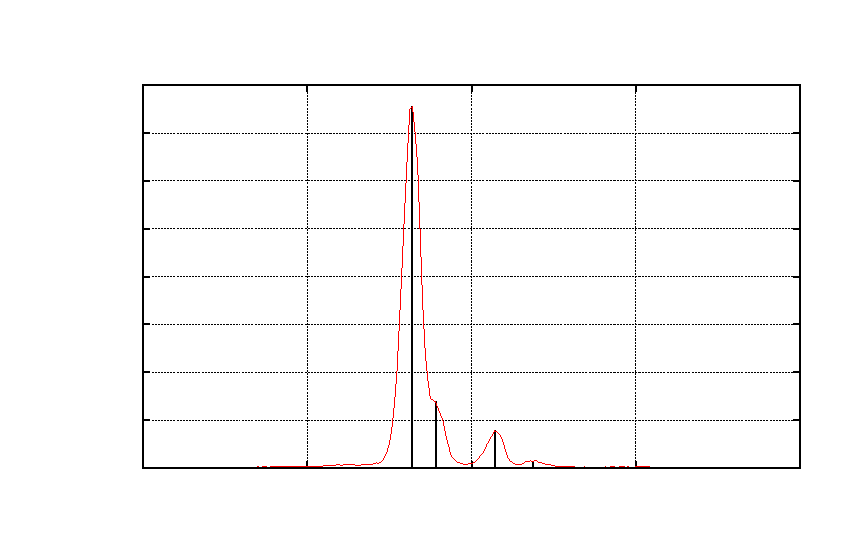
\includegraphics{./plots/kalibrierung}}%
    \gplfronttext
  \end{picture}%
\endgroup

\caption{Aufgenommenes Spektrum des Kalibriertargets (FeZn)}
\label{fig:kalibrierung}
\end{figure}

\subsection{Auswertung}
\subsubsection{Energieeichung durch das charakteristische FeZn-Spektrum}
Wie schon in Abschnitt \ref{sec:energiedetektor} besprochen, sind uns die Proportionalitäten sowie die Nullpunktsverschiebung des Röntgenenergiedetektors unbekannt.
Anhand des bekannten charakteristischen Spektrums\footnote{Aus dem \emph{X-Ray Data Booklet}\cite{booklet}} des FeZn-Plättchens kann nach dem Anpassen einer Eichgerade:
\begin{align}
  E(n) &= \Delta E \cdot n + E_\mathrm{Offset}
  \label{eq:eichgerade}
\end{align}
jedem \emph{Bin} $n$ die Energie $E$ zugeordnet werden.

Um die Eichgerade aus dem aufgenommenen Spektrum zu berechnen, identifizieren wir zunächst die $K_\alpha$- und $K_\beta$-Linien von Eisen und Zink (in Abbildung \ref{fig:kalibrierung} bereits geschehen).
Leider konnte die $K_\beta$-Linie von Eisen nicht gut aufgelöst werden.
Nun bestimmen wir die Peakschwerpunkte optisch, wobei wir für die beiden $\beta$-Linien etwas größere Fehler schätzen, da diese nicht sehr scharf sind.
Schließlich ordnen wir jeder Linie ihren Literaturwert zu und erhalten die Tabelle \ref{tab:eichgerade}.
\begin{table}[h]
\centering
\begin{tabular}{lSSS}
\toprule

{Linie} & {$n$} & {$E_\mathrm{Lit.} / \si{\electronvolt}$ \cite{booklet}}\\

\midrule

$K_\alpha(\mathrm{Fe})$ & 105 +- 1 & 6403.8 \\
$K_\beta(\mathrm{Fe})$ & 114 +- 2 & 7058.0 \\
$K_\alpha(\mathrm{Zn})$ & 137 +- 1 & 8638.9 \\
$K_\beta(\mathrm{Zn})$ & 152 +- 2 & 9572.0 \\

\bottomrule
\end{tabular}
\caption{Peakbestimmung}
\label{tab:eichgerade}
\end{table}

Anschließend tragen wir die Linenenergie $E_\mathrm{Lit.}$ der Linien gegen ihren Peakschwerpunkt $n$ auf und passen eine Gerade an die Messwerte an.
Wir erhalten für die Parameter der Gleichung \ref{eq:eichgerade}:
\begin{align}
  \Delta E &= \SI{67,53 +- 1,27}{\electronvolt}\\
  E_\mathrm{Offset} &= \SI{-657 +- 162}{\electronvolt}
\end{align}
Die Datenpunkte und die angepasste Gerade wurden in Abbildung \ref{fig:energieeichung} aufgetragen und legen (in Anbetracht der Messfehler) einen passablen Fit nahe.

\begin{figure}[h]
\centering
% GNUPLOT: LaTeX picture with Postscript
\begingroup
  \makeatletter
  \providecommand\color[2][]{%
    \GenericError{(gnuplot) \space\space\space\@spaces}{%
      Package color not loaded in conjunction with
      terminal option `colourtext'%
    }{See the gnuplot documentation for explanation.%
    }{Either use 'blacktext' in gnuplot or load the package
      color.sty in LaTeX.}%
    \renewcommand\color[2][]{}%
  }%
  \providecommand\includegraphics[2][]{%
    \GenericError{(gnuplot) \space\space\space\@spaces}{%
      Package graphicx or graphics not loaded%
    }{See the gnuplot documentation for explanation.%
    }{The gnuplot epslatex terminal needs graphicx.sty or graphics.sty.}%
    \renewcommand\includegraphics[2][]{}%
  }%
  \providecommand\rotatebox[2]{#2}%
  \@ifundefined{ifGPcolor}{%
    \newif\ifGPcolor
    \GPcolortrue
  }{}%
  \@ifundefined{ifGPblacktext}{%
    \newif\ifGPblacktext
    \GPblacktexttrue
  }{}%
  % define a \g@addto@macro without @ in the name:
  \let\gplgaddtomacro\g@addto@macro
  % define empty templates for all commands taking text:
  \gdef\gplbacktext{}%
  \gdef\gplfronttext{}%
  \makeatother
  \ifGPblacktext
    % no textcolor at all
    \def\colorrgb#1{}%
    \def\colorgray#1{}%
  \else
    % gray or color?
    \ifGPcolor
      \def\colorrgb#1{\color[rgb]{#1}}%
      \def\colorgray#1{\color[gray]{#1}}%
      \expandafter\def\csname LTw\endcsname{\color{white}}%
      \expandafter\def\csname LTb\endcsname{\color{black}}%
      \expandafter\def\csname LTa\endcsname{\color{black}}%
      \expandafter\def\csname LT0\endcsname{\color[rgb]{1,0,0}}%
      \expandafter\def\csname LT1\endcsname{\color[rgb]{0,1,0}}%
      \expandafter\def\csname LT2\endcsname{\color[rgb]{0,0,1}}%
      \expandafter\def\csname LT3\endcsname{\color[rgb]{1,0,1}}%
      \expandafter\def\csname LT4\endcsname{\color[rgb]{0,1,1}}%
      \expandafter\def\csname LT5\endcsname{\color[rgb]{1,1,0}}%
      \expandafter\def\csname LT6\endcsname{\color[rgb]{0,0,0}}%
      \expandafter\def\csname LT7\endcsname{\color[rgb]{1,0.3,0}}%
      \expandafter\def\csname LT8\endcsname{\color[rgb]{0.5,0.5,0.5}}%
    \else
      % gray
      \def\colorrgb#1{\color{black}}%
      \def\colorgray#1{\color[gray]{#1}}%
      \expandafter\def\csname LTw\endcsname{\color{white}}%
      \expandafter\def\csname LTb\endcsname{\color{black}}%
      \expandafter\def\csname LTa\endcsname{\color{black}}%
      \expandafter\def\csname LT0\endcsname{\color{black}}%
      \expandafter\def\csname LT1\endcsname{\color{black}}%
      \expandafter\def\csname LT2\endcsname{\color{black}}%
      \expandafter\def\csname LT3\endcsname{\color{black}}%
      \expandafter\def\csname LT4\endcsname{\color{black}}%
      \expandafter\def\csname LT5\endcsname{\color{black}}%
      \expandafter\def\csname LT6\endcsname{\color{black}}%
      \expandafter\def\csname LT7\endcsname{\color{black}}%
      \expandafter\def\csname LT8\endcsname{\color{black}}%
    \fi
  \fi
  \setlength{\unitlength}{0.0500bp}%
  \begin{picture}(7920.00,5040.00)%
    \gplgaddtomacro\gplbacktext{%
      \csname LTb\endcsname%
      \put(1210,704){\makebox(0,0)[r]{\strut{} 6000}}%
      \csname LTb\endcsname%
      \put(1210,1156){\makebox(0,0)[r]{\strut{} 6500}}%
      \csname LTb\endcsname%
      \put(1210,1609){\makebox(0,0)[r]{\strut{} 7000}}%
      \csname LTb\endcsname%
      \put(1210,2061){\makebox(0,0)[r]{\strut{} 7500}}%
      \csname LTb\endcsname%
      \put(1210,2513){\makebox(0,0)[r]{\strut{} 8000}}%
      \csname LTb\endcsname%
      \put(1210,2966){\makebox(0,0)[r]{\strut{} 8500}}%
      \csname LTb\endcsname%
      \put(1210,3418){\makebox(0,0)[r]{\strut{} 9000}}%
      \csname LTb\endcsname%
      \put(1210,3870){\makebox(0,0)[r]{\strut{} 9500}}%
      \csname LTb\endcsname%
      \put(1210,4323){\makebox(0,0)[r]{\strut{} 10000}}%
      \csname LTb\endcsname%
      \put(1210,4775){\makebox(0,0)[r]{\strut{} 10500}}%
      \csname LTb\endcsname%
      \put(1342,484){\makebox(0,0){\strut{} 100}}%
      \csname LTb\endcsname%
      \put(2372,484){\makebox(0,0){\strut{} 110}}%
      \csname LTb\endcsname%
      \put(3402,484){\makebox(0,0){\strut{} 120}}%
      \csname LTb\endcsname%
      \put(4432,484){\makebox(0,0){\strut{} 130}}%
      \csname LTb\endcsname%
      \put(5463,484){\makebox(0,0){\strut{} 140}}%
      \csname LTb\endcsname%
      \put(6493,484){\makebox(0,0){\strut{} 150}}%
      \csname LTb\endcsname%
      \put(7523,484){\makebox(0,0){\strut{} 160}}%
      \put(176,2739){\rotatebox{-270}{\makebox(0,0){\strut{}Energie $E / \si{\electronvolt}$}}}%
      \put(4432,154){\makebox(0,0){\strut{}Kanalnummer}}%
    }%
    \gplgaddtomacro\gplfronttext{%
      \csname LTb\endcsname%
      \put(2662,4602){\makebox(0,0)[r]{\strut{}Eichwerte}}%
      \csname LTb\endcsname%
      \put(2662,4382){\makebox(0,0)[r]{\strut{}Fitgerade}}%
    }%
    \gplbacktext
    \put(0,0){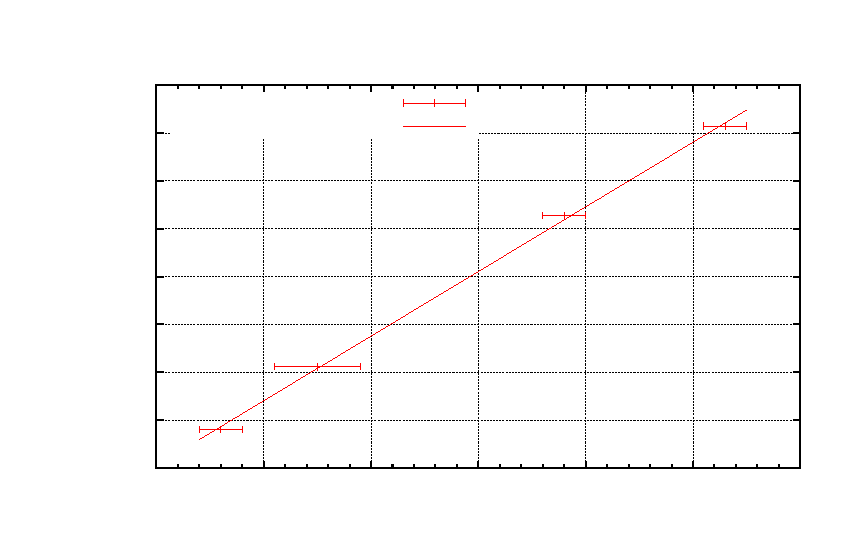
\includegraphics{./plots/energieeichung}}%
    \gplfronttext
  \end{picture}%
\endgroup

\caption{Zuordnung der Energien zu den Kanalnummern}
\label{fig:energieeichung}
\end{figure}

\clearpage

\subsubsection{Bestimmung der Komponenten der Legierungen}

Wir vergleichen nun die aufgenommenen Spektren der Proben mit denen der Referenzmessungen.
Anhand der Lage (und teilweise auch der Höhe) der Peaks kann so ausgesagt werden, welche Metalle zu welchen Anteilen in den Legierungen enthalten sind.
Zur Bestimmung der Elemente in der Legierung reicht dabei aus, Übereinstimmungen der Lage der Peaks in Proben- und Referenzspektrum zu finden, solange die Größenordnung der Höhen übereinstimmt.
Zur Bestimmung der Masseanteile gemäß (\ref{eq:masseanteile}) muss weiterhin auch noch die Höhe der Peaks gemessen werden.

Bei Probe 1 finden wir so durch Vergleich mit dem Referenzspektrum (s. Anhang \ref{sec:referenzspektren}), dass das höchste Peak Eisen entspricht.
Dieser Peak wird dabei noch überlagert von einem Peak aus dem Nickelspektrum, so dass wir dieses als zweite Komponente identifizieren können.
Der flache Peak bei ca. \SI{10}{\kilo\electronvolt} gehört auch zu Eisen, wir finden ihn auch im Referenzspektrum.
Das weiter links liegende Peak kann mit der abgelesenen Energie und \cite{booklet} zu Chrom bestimmt werden.
Bei genauem Hinsehen fällt auf, dass es sich hierbei um eine Doppellinie handelt, da die Spitze des Peaks nicht scharf ausgeprägt ist.

\begin{figure}[h]
\centering
% GNUPLOT: LaTeX picture with Postscript
\begingroup
  \makeatletter
  \providecommand\color[2][]{%
    \GenericError{(gnuplot) \space\space\space\@spaces}{%
      Package color not loaded in conjunction with
      terminal option `colourtext'%
    }{See the gnuplot documentation for explanation.%
    }{Either use 'blacktext' in gnuplot or load the package
      color.sty in LaTeX.}%
    \renewcommand\color[2][]{}%
  }%
  \providecommand\includegraphics[2][]{%
    \GenericError{(gnuplot) \space\space\space\@spaces}{%
      Package graphicx or graphics not loaded%
    }{See the gnuplot documentation for explanation.%
    }{The gnuplot epslatex terminal needs graphicx.sty or graphics.sty.}%
    \renewcommand\includegraphics[2][]{}%
  }%
  \providecommand\rotatebox[2]{#2}%
  \@ifundefined{ifGPcolor}{%
    \newif\ifGPcolor
    \GPcolortrue
  }{}%
  \@ifundefined{ifGPblacktext}{%
    \newif\ifGPblacktext
    \GPblacktexttrue
  }{}%
  % define a \g@addto@macro without @ in the name:
  \let\gplgaddtomacro\g@addto@macro
  % define empty templates for all commands taking text:
  \gdef\gplbacktext{}%
  \gdef\gplfronttext{}%
  \makeatother
  \ifGPblacktext
    % no textcolor at all
    \def\colorrgb#1{}%
    \def\colorgray#1{}%
  \else
    % gray or color?
    \ifGPcolor
      \def\colorrgb#1{\color[rgb]{#1}}%
      \def\colorgray#1{\color[gray]{#1}}%
      \expandafter\def\csname LTw\endcsname{\color{white}}%
      \expandafter\def\csname LTb\endcsname{\color{black}}%
      \expandafter\def\csname LTa\endcsname{\color{black}}%
      \expandafter\def\csname LT0\endcsname{\color[rgb]{1,0,0}}%
      \expandafter\def\csname LT1\endcsname{\color[rgb]{0,1,0}}%
      \expandafter\def\csname LT2\endcsname{\color[rgb]{0,0,1}}%
      \expandafter\def\csname LT3\endcsname{\color[rgb]{1,0,1}}%
      \expandafter\def\csname LT4\endcsname{\color[rgb]{0,1,1}}%
      \expandafter\def\csname LT5\endcsname{\color[rgb]{1,1,0}}%
      \expandafter\def\csname LT6\endcsname{\color[rgb]{0,0,0}}%
      \expandafter\def\csname LT7\endcsname{\color[rgb]{1,0.3,0}}%
      \expandafter\def\csname LT8\endcsname{\color[rgb]{0.5,0.5,0.5}}%
    \else
      % gray
      \def\colorrgb#1{\color{black}}%
      \def\colorgray#1{\color[gray]{#1}}%
      \expandafter\def\csname LTw\endcsname{\color{white}}%
      \expandafter\def\csname LTb\endcsname{\color{black}}%
      \expandafter\def\csname LTa\endcsname{\color{black}}%
      \expandafter\def\csname LT0\endcsname{\color{black}}%
      \expandafter\def\csname LT1\endcsname{\color{black}}%
      \expandafter\def\csname LT2\endcsname{\color{black}}%
      \expandafter\def\csname LT3\endcsname{\color{black}}%
      \expandafter\def\csname LT4\endcsname{\color{black}}%
      \expandafter\def\csname LT5\endcsname{\color{black}}%
      \expandafter\def\csname LT6\endcsname{\color{black}}%
      \expandafter\def\csname LT7\endcsname{\color{black}}%
      \expandafter\def\csname LT8\endcsname{\color{black}}%
    \fi
  \fi
  \setlength{\unitlength}{0.0500bp}%
  \begin{picture}(7920.00,5040.00)%
    \gplgaddtomacro\gplbacktext{%
      \csname LTb\endcsname%
      \put(1078,704){\makebox(0,0)[r]{\strut{} 0}}%
      \csname LTb\endcsname%
      \put(1078,1166){\makebox(0,0)[r]{\strut{} 1000}}%
      \csname LTb\endcsname%
      \put(1078,1628){\makebox(0,0)[r]{\strut{} 2000}}%
      \csname LTb\endcsname%
      \put(1078,2090){\makebox(0,0)[r]{\strut{} 3000}}%
      \csname LTb\endcsname%
      \put(1078,2553){\makebox(0,0)[r]{\strut{} 4000}}%
      \csname LTb\endcsname%
      \put(1078,3015){\makebox(0,0)[r]{\strut{} 5000}}%
      \csname LTb\endcsname%
      \put(1078,3477){\makebox(0,0)[r]{\strut{} 6000}}%
      \csname LTb\endcsname%
      \put(1078,3939){\makebox(0,0)[r]{\strut{} 7000}}%
      \csname LTb\endcsname%
      \put(1210,484){\makebox(0,0){\strut{} 0}}%
      \csname LTb\endcsname%
      \put(2788,484){\makebox(0,0){\strut{} 64}}%
      \csname LTb\endcsname%
      \put(4367,484){\makebox(0,0){\strut{} 128}}%
      \csname LTb\endcsname%
      \put(5945,484){\makebox(0,0){\strut{} 192}}%
      \csname LTb\endcsname%
      \put(7523,484){\makebox(0,0){\strut{} 256}}%
      \csname LTb\endcsname%
      \put(1450,4159){\makebox(0,0){\strut{} 0}}%
      \csname LTb\endcsname%
      \put(3276,4159){\makebox(0,0){\strut{} 5}}%
      \csname LTb\endcsname%
      \put(5102,4159){\makebox(0,0){\strut{} 10}}%
      \csname LTb\endcsname%
      \put(6928,4159){\makebox(0,0){\strut{} 15}}%
      \put(176,2321){\rotatebox{-270}{\makebox(0,0){\strut{}Counts}}}%
      \put(4366,154){\makebox(0,0){\strut{}Kanalnummer}}%
      \put(4366,4929){\makebox(0,0){\strut{}Spektrum von Probe 1}}%
      \put(4366,4488){\makebox(0,0){\strut{}Energie / $\si{\kilo\electronvolt}$}}%
    }%
    \gplgaddtomacro\gplfronttext{%
    }%
    \gplbacktext
    \put(0,0){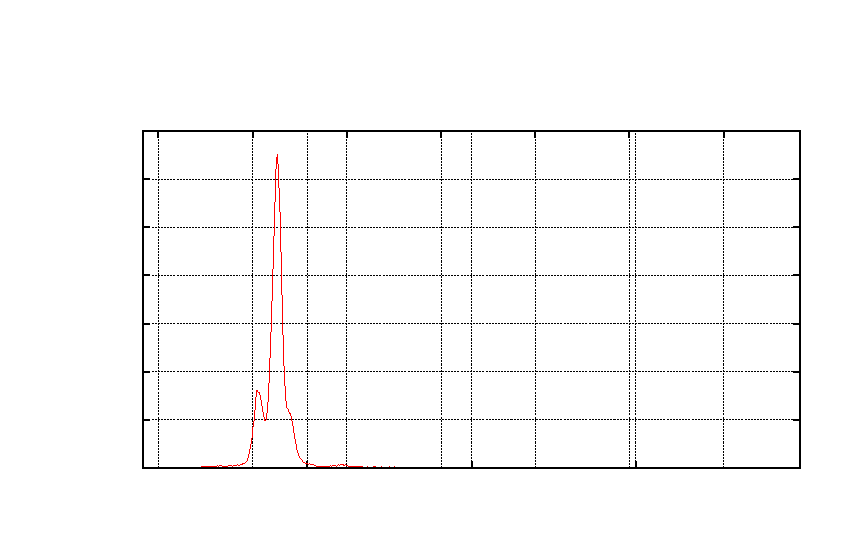
\includegraphics{./plots/probe1}}%
    \gplfronttext
  \end{picture}%
\endgroup

\caption{Probe 1}
\label{fig:probe1}
\end{figure}

Für Probe 2 finden wir so eine Legierung von Kupfer und Zink, was auf Messing schließen lässt.
Auffallend ist dabei der hohe, schmale Peak des Kupferspektrums und der nah daran liegende Peak von Zink.
Die Höhen der jeweiligen Peaks addieren sich durch teilweise Überlagerungen der Spektren, da die Peaks sehr nah beieinander liegen.

\begin{figure}[!h]
\centering
% GNUPLOT: LaTeX picture with Postscript
\begingroup
  \makeatletter
  \providecommand\color[2][]{%
    \GenericError{(gnuplot) \space\space\space\@spaces}{%
      Package color not loaded in conjunction with
      terminal option `colourtext'%
    }{See the gnuplot documentation for explanation.%
    }{Either use 'blacktext' in gnuplot or load the package
      color.sty in LaTeX.}%
    \renewcommand\color[2][]{}%
  }%
  \providecommand\includegraphics[2][]{%
    \GenericError{(gnuplot) \space\space\space\@spaces}{%
      Package graphicx or graphics not loaded%
    }{See the gnuplot documentation for explanation.%
    }{The gnuplot epslatex terminal needs graphicx.sty or graphics.sty.}%
    \renewcommand\includegraphics[2][]{}%
  }%
  \providecommand\rotatebox[2]{#2}%
  \@ifundefined{ifGPcolor}{%
    \newif\ifGPcolor
    \GPcolortrue
  }{}%
  \@ifundefined{ifGPblacktext}{%
    \newif\ifGPblacktext
    \GPblacktexttrue
  }{}%
  % define a \g@addto@macro without @ in the name:
  \let\gplgaddtomacro\g@addto@macro
  % define empty templates for all commands taking text:
  \gdef\gplbacktext{}%
  \gdef\gplfronttext{}%
  \makeatother
  \ifGPblacktext
    % no textcolor at all
    \def\colorrgb#1{}%
    \def\colorgray#1{}%
  \else
    % gray or color?
    \ifGPcolor
      \def\colorrgb#1{\color[rgb]{#1}}%
      \def\colorgray#1{\color[gray]{#1}}%
      \expandafter\def\csname LTw\endcsname{\color{white}}%
      \expandafter\def\csname LTb\endcsname{\color{black}}%
      \expandafter\def\csname LTa\endcsname{\color{black}}%
      \expandafter\def\csname LT0\endcsname{\color[rgb]{1,0,0}}%
      \expandafter\def\csname LT1\endcsname{\color[rgb]{0,1,0}}%
      \expandafter\def\csname LT2\endcsname{\color[rgb]{0,0,1}}%
      \expandafter\def\csname LT3\endcsname{\color[rgb]{1,0,1}}%
      \expandafter\def\csname LT4\endcsname{\color[rgb]{0,1,1}}%
      \expandafter\def\csname LT5\endcsname{\color[rgb]{1,1,0}}%
      \expandafter\def\csname LT6\endcsname{\color[rgb]{0,0,0}}%
      \expandafter\def\csname LT7\endcsname{\color[rgb]{1,0.3,0}}%
      \expandafter\def\csname LT8\endcsname{\color[rgb]{0.5,0.5,0.5}}%
    \else
      % gray
      \def\colorrgb#1{\color{black}}%
      \def\colorgray#1{\color[gray]{#1}}%
      \expandafter\def\csname LTw\endcsname{\color{white}}%
      \expandafter\def\csname LTb\endcsname{\color{black}}%
      \expandafter\def\csname LTa\endcsname{\color{black}}%
      \expandafter\def\csname LT0\endcsname{\color{black}}%
      \expandafter\def\csname LT1\endcsname{\color{black}}%
      \expandafter\def\csname LT2\endcsname{\color{black}}%
      \expandafter\def\csname LT3\endcsname{\color{black}}%
      \expandafter\def\csname LT4\endcsname{\color{black}}%
      \expandafter\def\csname LT5\endcsname{\color{black}}%
      \expandafter\def\csname LT6\endcsname{\color{black}}%
      \expandafter\def\csname LT7\endcsname{\color{black}}%
      \expandafter\def\csname LT8\endcsname{\color{black}}%
    \fi
  \fi
  \setlength{\unitlength}{0.0500bp}%
  \begin{picture}(7920.00,5040.00)%
    \gplgaddtomacro\gplbacktext{%
      \csname LTb\endcsname%
      \put(1078,704){\makebox(0,0)[r]{\strut{} 0}}%
      \csname LTb\endcsname%
      \put(1078,1243){\makebox(0,0)[r]{\strut{} 500}}%
      \csname LTb\endcsname%
      \put(1078,1782){\makebox(0,0)[r]{\strut{} 1000}}%
      \csname LTb\endcsname%
      \put(1078,2322){\makebox(0,0)[r]{\strut{} 1500}}%
      \csname LTb\endcsname%
      \put(1078,2861){\makebox(0,0)[r]{\strut{} 2000}}%
      \csname LTb\endcsname%
      \put(1078,3400){\makebox(0,0)[r]{\strut{} 2500}}%
      \csname LTb\endcsname%
      \put(1078,3939){\makebox(0,0)[r]{\strut{} 3000}}%
      \csname LTb\endcsname%
      \put(1210,484){\makebox(0,0){\strut{} 0}}%
      \csname LTb\endcsname%
      \put(2788,484){\makebox(0,0){\strut{} 128}}%
      \csname LTb\endcsname%
      \put(4367,484){\makebox(0,0){\strut{} 256}}%
      \csname LTb\endcsname%
      \put(5945,484){\makebox(0,0){\strut{} 384}}%
      \csname LTb\endcsname%
      \put(7523,484){\makebox(0,0){\strut{} 512}}%
      \csname LTb\endcsname%
      \put(1360,4159){\makebox(0,0){\strut{} 0}}%
      \csname LTb\endcsname%
      \put(2265,4159){\makebox(0,0){\strut{} 5}}%
      \csname LTb\endcsname%
      \put(3169,4159){\makebox(0,0){\strut{} 10}}%
      \csname LTb\endcsname%
      \put(4074,4159){\makebox(0,0){\strut{} 15}}%
      \csname LTb\endcsname%
      \put(4978,4159){\makebox(0,0){\strut{} 20}}%
      \csname LTb\endcsname%
      \put(5883,4159){\makebox(0,0){\strut{} 25}}%
      \csname LTb\endcsname%
      \put(6787,4159){\makebox(0,0){\strut{} 30}}%
      \put(176,2321){\rotatebox{-270}{\makebox(0,0){\strut{}Counts}}}%
      \put(4366,154){\makebox(0,0){\strut{}Kanalnummer}}%
      \put(4366,4929){\makebox(0,0){\strut{}Spektrum von Probe 2}}%
      \put(4366,4488){\makebox(0,0){\strut{}Energie / $\si{\kilo\electronvolt}$}}%
    }%
    \gplgaddtomacro\gplfronttext{%
    }%
    \gplbacktext
    \put(0,0){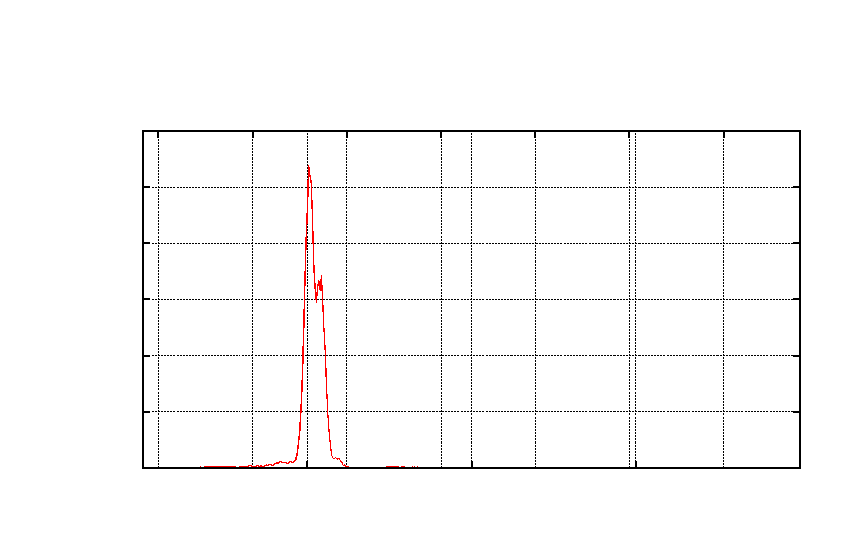
\includegraphics{./plots/probe2}}%
    \gplfronttext
  \end{picture}%
\endgroup

\caption{Probe 2}
\label{fig:probe2}
\end{figure}

Probe 3 weist ein sehr ähnliches Spektrum wie Probe 2 auf mit (bis auf die Höhen der Peaks) gleichen Charakteristika, so dass wir auch hier Kupfer und Zink als Hauptbestandteile der Legierung bestimmen.

\begin{figure}[!h]
\centering
% GNUPLOT: LaTeX picture with Postscript
\begingroup
  \makeatletter
  \providecommand\color[2][]{%
    \GenericError{(gnuplot) \space\space\space\@spaces}{%
      Package color not loaded in conjunction with
      terminal option `colourtext'%
    }{See the gnuplot documentation for explanation.%
    }{Either use 'blacktext' in gnuplot or load the package
      color.sty in LaTeX.}%
    \renewcommand\color[2][]{}%
  }%
  \providecommand\includegraphics[2][]{%
    \GenericError{(gnuplot) \space\space\space\@spaces}{%
      Package graphicx or graphics not loaded%
    }{See the gnuplot documentation for explanation.%
    }{The gnuplot epslatex terminal needs graphicx.sty or graphics.sty.}%
    \renewcommand\includegraphics[2][]{}%
  }%
  \providecommand\rotatebox[2]{#2}%
  \@ifundefined{ifGPcolor}{%
    \newif\ifGPcolor
    \GPcolortrue
  }{}%
  \@ifundefined{ifGPblacktext}{%
    \newif\ifGPblacktext
    \GPblacktexttrue
  }{}%
  % define a \g@addto@macro without @ in the name:
  \let\gplgaddtomacro\g@addto@macro
  % define empty templates for all commands taking text:
  \gdef\gplbacktext{}%
  \gdef\gplfronttext{}%
  \makeatother
  \ifGPblacktext
    % no textcolor at all
    \def\colorrgb#1{}%
    \def\colorgray#1{}%
  \else
    % gray or color?
    \ifGPcolor
      \def\colorrgb#1{\color[rgb]{#1}}%
      \def\colorgray#1{\color[gray]{#1}}%
      \expandafter\def\csname LTw\endcsname{\color{white}}%
      \expandafter\def\csname LTb\endcsname{\color{black}}%
      \expandafter\def\csname LTa\endcsname{\color{black}}%
      \expandafter\def\csname LT0\endcsname{\color[rgb]{1,0,0}}%
      \expandafter\def\csname LT1\endcsname{\color[rgb]{0,1,0}}%
      \expandafter\def\csname LT2\endcsname{\color[rgb]{0,0,1}}%
      \expandafter\def\csname LT3\endcsname{\color[rgb]{1,0,1}}%
      \expandafter\def\csname LT4\endcsname{\color[rgb]{0,1,1}}%
      \expandafter\def\csname LT5\endcsname{\color[rgb]{1,1,0}}%
      \expandafter\def\csname LT6\endcsname{\color[rgb]{0,0,0}}%
      \expandafter\def\csname LT7\endcsname{\color[rgb]{1,0.3,0}}%
      \expandafter\def\csname LT8\endcsname{\color[rgb]{0.5,0.5,0.5}}%
    \else
      % gray
      \def\colorrgb#1{\color{black}}%
      \def\colorgray#1{\color[gray]{#1}}%
      \expandafter\def\csname LTw\endcsname{\color{white}}%
      \expandafter\def\csname LTb\endcsname{\color{black}}%
      \expandafter\def\csname LTa\endcsname{\color{black}}%
      \expandafter\def\csname LT0\endcsname{\color{black}}%
      \expandafter\def\csname LT1\endcsname{\color{black}}%
      \expandafter\def\csname LT2\endcsname{\color{black}}%
      \expandafter\def\csname LT3\endcsname{\color{black}}%
      \expandafter\def\csname LT4\endcsname{\color{black}}%
      \expandafter\def\csname LT5\endcsname{\color{black}}%
      \expandafter\def\csname LT6\endcsname{\color{black}}%
      \expandafter\def\csname LT7\endcsname{\color{black}}%
      \expandafter\def\csname LT8\endcsname{\color{black}}%
    \fi
  \fi
  \setlength{\unitlength}{0.0500bp}%
  \begin{picture}(7920.00,5040.00)%
    \gplgaddtomacro\gplbacktext{%
      \csname LTb\endcsname%
      \put(1078,704){\makebox(0,0)[r]{\strut{} 0}}%
      \csname LTb\endcsname%
      \put(1078,1351){\makebox(0,0)[r]{\strut{} 500}}%
      \csname LTb\endcsname%
      \put(1078,1998){\makebox(0,0)[r]{\strut{} 1000}}%
      \csname LTb\endcsname%
      \put(1078,2645){\makebox(0,0)[r]{\strut{} 1500}}%
      \csname LTb\endcsname%
      \put(1078,3292){\makebox(0,0)[r]{\strut{} 2000}}%
      \csname LTb\endcsname%
      \put(1078,3939){\makebox(0,0)[r]{\strut{} 2500}}%
      \csname LTb\endcsname%
      \put(1210,484){\makebox(0,0){\strut{} 64}}%
      \csname LTb\endcsname%
      \put(2473,484){\makebox(0,0){\strut{} 96}}%
      \csname LTb\endcsname%
      \put(3735,484){\makebox(0,0){\strut{} 128}}%
      \csname LTb\endcsname%
      \put(4998,484){\makebox(0,0){\strut{} 160}}%
      \csname LTb\endcsname%
      \put(6260,484){\makebox(0,0){\strut{} 192}}%
      \csname LTb\endcsname%
      \put(7523,484){\makebox(0,0){\strut{} 224}}%
      \csname LTb\endcsname%
      \put(1406,4159){\makebox(0,0){\strut{} 4}}%
      \csname LTb\endcsname%
      \put(2575,4159){\makebox(0,0){\strut{} 6}}%
      \csname LTb\endcsname%
      \put(3743,4159){\makebox(0,0){\strut{} 8}}%
      \csname LTb\endcsname%
      \put(4912,4159){\makebox(0,0){\strut{} 10}}%
      \csname LTb\endcsname%
      \put(6080,4159){\makebox(0,0){\strut{} 12}}%
      \csname LTb\endcsname%
      \put(7248,4159){\makebox(0,0){\strut{} 14}}%
      \put(176,2321){\rotatebox{-270}{\makebox(0,0){\strut{}Counts}}}%
      \put(4366,154){\makebox(0,0){\strut{}Kanalnummer}}%
      \put(4366,4929){\makebox(0,0){\strut{}Spektrum von Probe 3}}%
      \put(4366,4488){\makebox(0,0){\strut{}Energie / $\si{\kilo\electronvolt}$}}%
      \put(3861,3777){\makebox(0,0)[l]{\strut{}K$_{\alpha}$(Cu)}}%
      \put(4177,2969){\makebox(0,0)[l]{\strut{}K$_{\alpha}$(Zn)}}%
      \put(4682,930){\makebox(0,0)[l]{\strut{}K$_{\beta}$(Zn)}}%
    }%
    \gplgaddtomacro\gplfronttext{%
    }%
    \gplbacktext
    \put(0,0){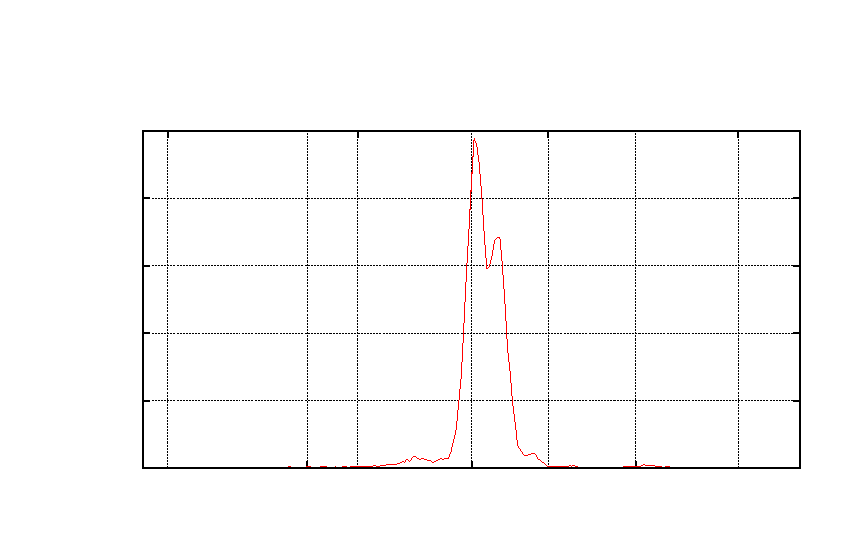
\includegraphics{./plots/probe3}}%
    \gplfronttext
  \end{picture}%
\endgroup

\caption{Probe 3}
\label{fig:probe3}
\end{figure}

\begin{figure}[h]
\centering
% GNUPLOT: LaTeX picture with Postscript
\begingroup
  \makeatletter
  \providecommand\color[2][]{%
    \GenericError{(gnuplot) \space\space\space\@spaces}{%
      Package color not loaded in conjunction with
      terminal option `colourtext'%
    }{See the gnuplot documentation for explanation.%
    }{Either use 'blacktext' in gnuplot or load the package
      color.sty in LaTeX.}%
    \renewcommand\color[2][]{}%
  }%
  \providecommand\includegraphics[2][]{%
    \GenericError{(gnuplot) \space\space\space\@spaces}{%
      Package graphicx or graphics not loaded%
    }{See the gnuplot documentation for explanation.%
    }{The gnuplot epslatex terminal needs graphicx.sty or graphics.sty.}%
    \renewcommand\includegraphics[2][]{}%
  }%
  \providecommand\rotatebox[2]{#2}%
  \@ifundefined{ifGPcolor}{%
    \newif\ifGPcolor
    \GPcolortrue
  }{}%
  \@ifundefined{ifGPblacktext}{%
    \newif\ifGPblacktext
    \GPblacktexttrue
  }{}%
  % define a \g@addto@macro without @ in the name:
  \let\gplgaddtomacro\g@addto@macro
  % define empty templates for all commands taking text:
  \gdef\gplbacktext{}%
  \gdef\gplfronttext{}%
  \makeatother
  \ifGPblacktext
    % no textcolor at all
    \def\colorrgb#1{}%
    \def\colorgray#1{}%
  \else
    % gray or color?
    \ifGPcolor
      \def\colorrgb#1{\color[rgb]{#1}}%
      \def\colorgray#1{\color[gray]{#1}}%
      \expandafter\def\csname LTw\endcsname{\color{white}}%
      \expandafter\def\csname LTb\endcsname{\color{black}}%
      \expandafter\def\csname LTa\endcsname{\color{black}}%
      \expandafter\def\csname LT0\endcsname{\color[rgb]{1,0,0}}%
      \expandafter\def\csname LT1\endcsname{\color[rgb]{0,1,0}}%
      \expandafter\def\csname LT2\endcsname{\color[rgb]{0,0,1}}%
      \expandafter\def\csname LT3\endcsname{\color[rgb]{1,0,1}}%
      \expandafter\def\csname LT4\endcsname{\color[rgb]{0,1,1}}%
      \expandafter\def\csname LT5\endcsname{\color[rgb]{1,1,0}}%
      \expandafter\def\csname LT6\endcsname{\color[rgb]{0,0,0}}%
      \expandafter\def\csname LT7\endcsname{\color[rgb]{1,0.3,0}}%
      \expandafter\def\csname LT8\endcsname{\color[rgb]{0.5,0.5,0.5}}%
    \else
      % gray
      \def\colorrgb#1{\color{black}}%
      \def\colorgray#1{\color[gray]{#1}}%
      \expandafter\def\csname LTw\endcsname{\color{white}}%
      \expandafter\def\csname LTb\endcsname{\color{black}}%
      \expandafter\def\csname LTa\endcsname{\color{black}}%
      \expandafter\def\csname LT0\endcsname{\color{black}}%
      \expandafter\def\csname LT1\endcsname{\color{black}}%
      \expandafter\def\csname LT2\endcsname{\color{black}}%
      \expandafter\def\csname LT3\endcsname{\color{black}}%
      \expandafter\def\csname LT4\endcsname{\color{black}}%
      \expandafter\def\csname LT5\endcsname{\color{black}}%
      \expandafter\def\csname LT6\endcsname{\color{black}}%
      \expandafter\def\csname LT7\endcsname{\color{black}}%
      \expandafter\def\csname LT8\endcsname{\color{black}}%
    \fi
  \fi
  \setlength{\unitlength}{0.0500bp}%
  \begin{picture}(7920.00,5040.00)%
    \gplgaddtomacro\gplbacktext{%
      \csname LTb\endcsname%
      \put(1078,704){\makebox(0,0)[r]{\strut{} 0}}%
      \csname LTb\endcsname%
      \put(1078,1243){\makebox(0,0)[r]{\strut{} 500}}%
      \csname LTb\endcsname%
      \put(1078,1782){\makebox(0,0)[r]{\strut{} 1000}}%
      \csname LTb\endcsname%
      \put(1078,2322){\makebox(0,0)[r]{\strut{} 1500}}%
      \csname LTb\endcsname%
      \put(1078,2861){\makebox(0,0)[r]{\strut{} 2000}}%
      \csname LTb\endcsname%
      \put(1078,3400){\makebox(0,0)[r]{\strut{} 2500}}%
      \csname LTb\endcsname%
      \put(1078,3939){\makebox(0,0)[r]{\strut{} 3000}}%
      \csname LTb\endcsname%
      \put(1210,484){\makebox(0,0){\strut{} 0}}%
      \csname LTb\endcsname%
      \put(2788,484){\makebox(0,0){\strut{} 128}}%
      \csname LTb\endcsname%
      \put(4367,484){\makebox(0,0){\strut{} 256}}%
      \csname LTb\endcsname%
      \put(5945,484){\makebox(0,0){\strut{} 384}}%
      \csname LTb\endcsname%
      \put(7523,484){\makebox(0,0){\strut{} 512}}%
      \csname LTb\endcsname%
      \put(1360,4159){\makebox(0,0){\strut{} 0}}%
      \csname LTb\endcsname%
      \put(2265,4159){\makebox(0,0){\strut{} 5}}%
      \csname LTb\endcsname%
      \put(3169,4159){\makebox(0,0){\strut{} 10}}%
      \csname LTb\endcsname%
      \put(4074,4159){\makebox(0,0){\strut{} 15}}%
      \csname LTb\endcsname%
      \put(4978,4159){\makebox(0,0){\strut{} 20}}%
      \csname LTb\endcsname%
      \put(5883,4159){\makebox(0,0){\strut{} 25}}%
      \csname LTb\endcsname%
      \put(6787,4159){\makebox(0,0){\strut{} 30}}%
      \put(176,2321){\rotatebox{-270}{\makebox(0,0){\strut{}Counts}}}%
      \put(4366,154){\makebox(0,0){\strut{}Kanalnummer}}%
      \put(4366,4929){\makebox(0,0){\strut{}Spektrum von Probe 4}}%
      \put(4366,4488){\makebox(0,0){\strut{}Energie / $\si{\kilo\electronvolt}$}}%
    }%
    \gplgaddtomacro\gplfronttext{%
    }%
    \gplbacktext
    \put(0,0){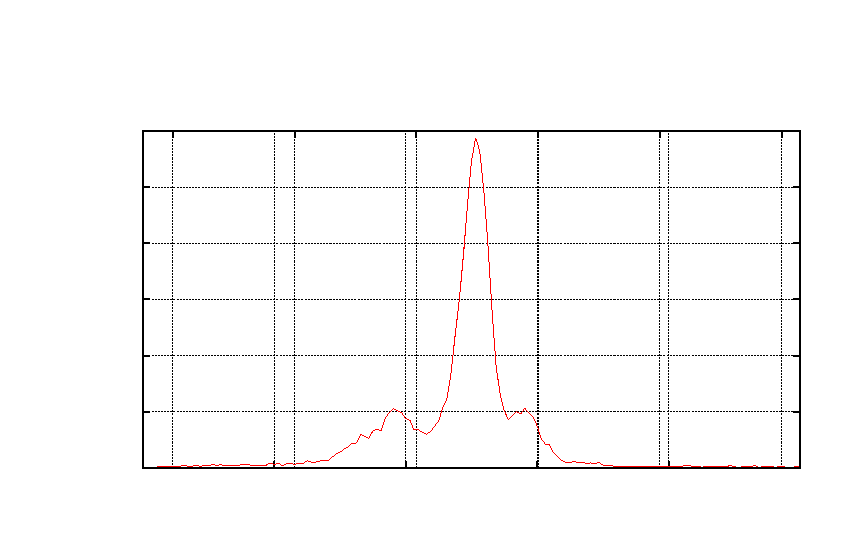
\includegraphics{./plots/probe4}}%
    \gplfronttext
  \end{picture}%
\endgroup

\caption{Probe 4}
\label{fig:probe4}
\end{figure}

\subsubsection{Massenanteile der Komponenten in Probe 1}

Wir wollen nun für eine Probe die Massenanteile der einzelnen Komponenten bestimmen und wählen dafür Probe 1 aus.

\begin{table}[h]
\centering
\begin{tabular}{p{6cm}|ll}
\toprule

Element 										& {Zink}	& {Kupfer} 	\\
Dichte $\rho$ / \si{\gram\per\cubic\centi\metre}& \num{7.14}& \num{8.92}\\
Höhe des (höchsten) Peaks $H$ / Counts			& 1671 		& 2689		\\
$\Delta H$ / Counts								& 84		& 135		\\
Referenzhöhe $H_0$ / Counts 					& 3758		& 3872		\\
$\Delta H_0$ / Counts							& 188		& 194		\\
Massenanteil									& {\SI{33,9+-2,3}{\percent}}&{\SI{66,1+-2,5}{\percent}}\\

\bottomrule
\end{tabular}
\caption{Massenanteile}
\label{tab:massenanteile}
\end{table}

\subsection{Diskussion}

\section{Versuchsteil 3: Laue-Aufnahme}
\subsection{Versuchsdurchführung}

\subsection{Messdaten}
\begin{figure}[h!]
\centering
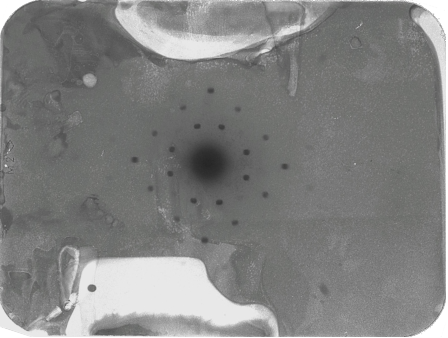
\includegraphics[width=0.60\textwidth]{./grafiken/film.pdf}
\caption{Scan des Röntgenfilms (Länge der langen Kante \SI{76 +- 0.5}{\milli\metre} auf \SI{895}{\pixel}}
\label{fig:film}
\end{figure}

\begin{figure}[h!]
\centering
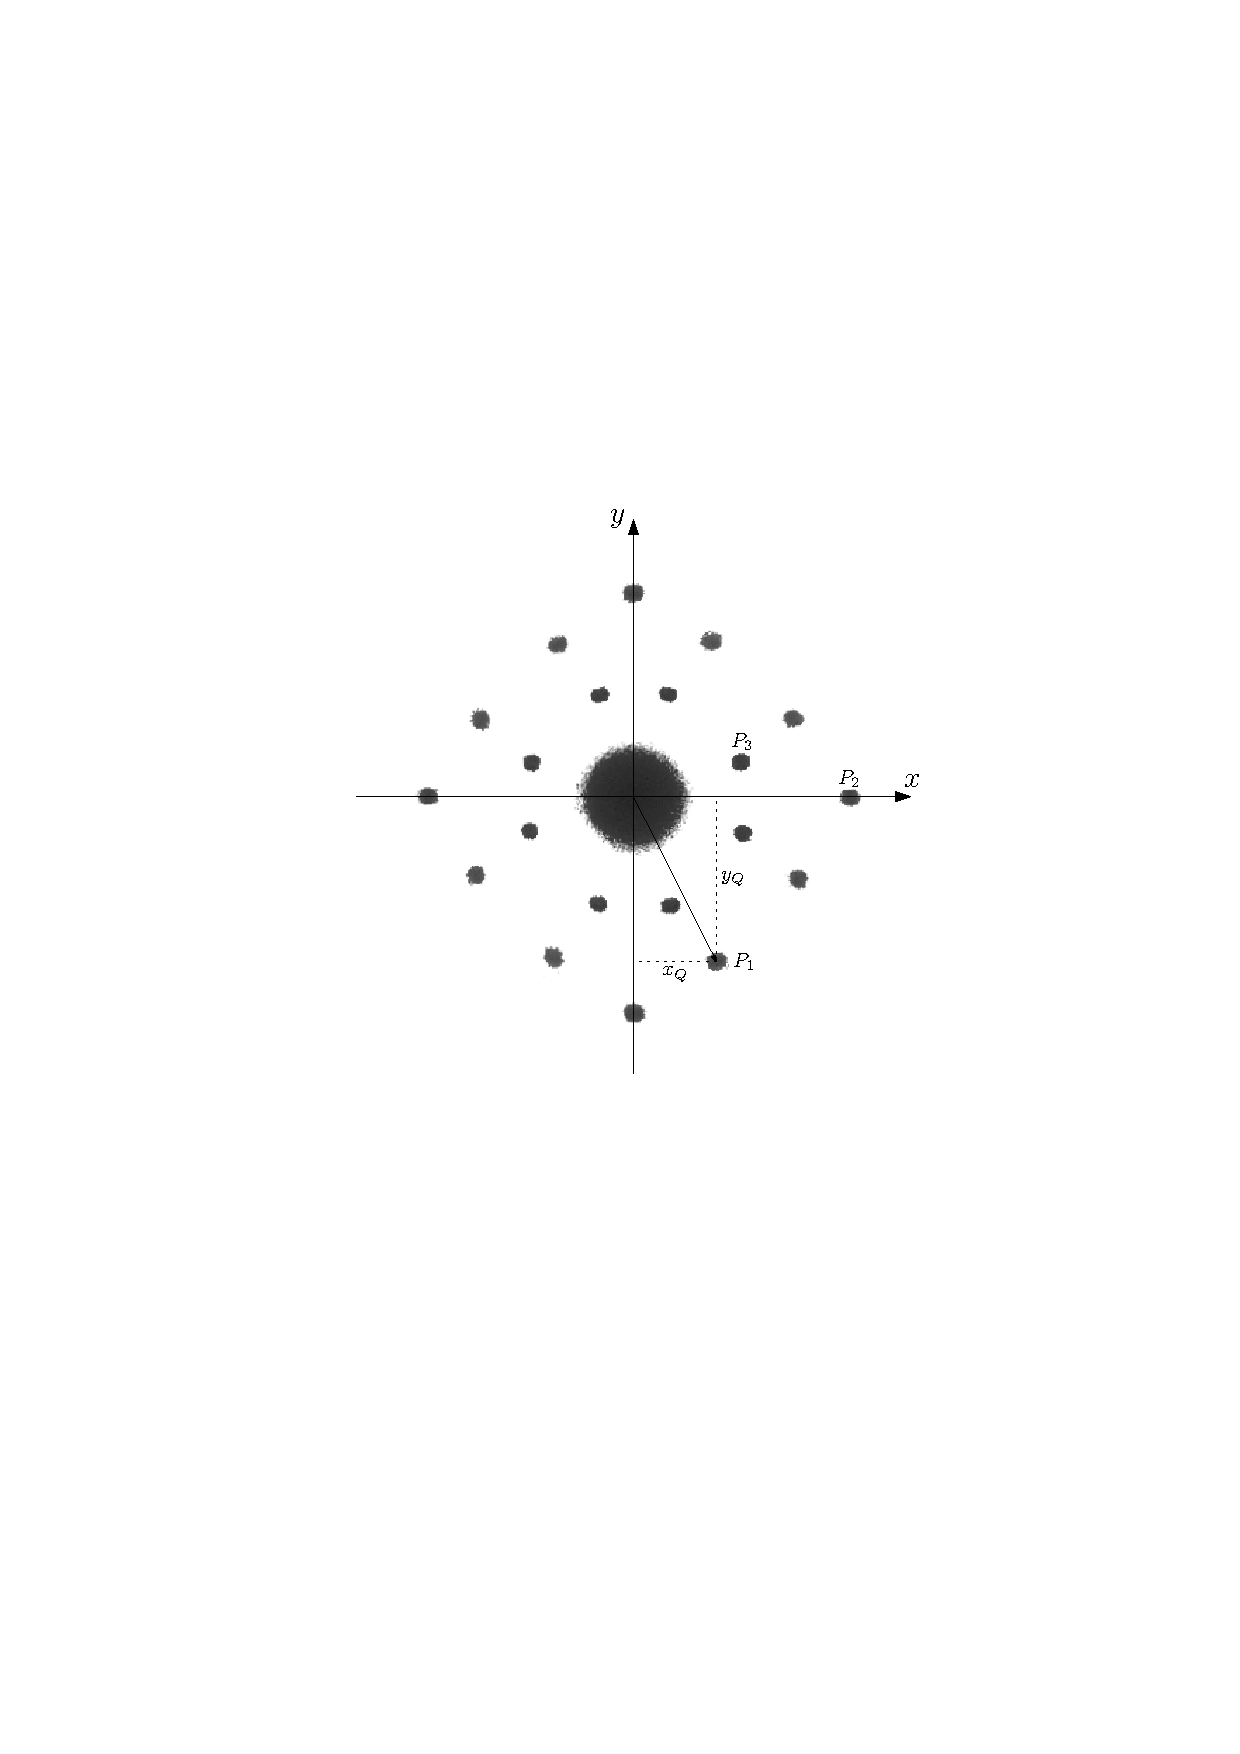
\includegraphics[width=0.9\textwidth]{./grafiken/film_koord.pdf}
\caption{bearbeiteter Ausschnitt des Röntgenfilms}
\label{fig:film_koord}
\end{figure}



\subsection{Auswertung}
\subsubsection{Bestimmung der verursachenden Netzebenenschar eines Laue-Reflexes}
Zunächst wurde der Röntgenfilm in Abbildung \ref{fig:film} mit einem Scanner digitalisiert.
Anschließend wurde das digitale Bild entsprechend bearbeitet, um Abbildung \ref{fig:film_koord} zu erhalten.
Dort messen wir mit digitalen Hilfsmitteln (\emph{Gimp}) die Koordinaten der Reflexe $P_1, P_2$ und $P_3$, welche wir auswerten wollen.
Die Koordinaten der Punkte wurden in Tabelle \ref{tab:laue_digi} in Pixeln angegeben.
\begin{table}[h]
\centering
\begin{tabular}{lSS}
\toprule

{\#} & {$x_Q / \si{\pixel}$} & {$y_Q / \si{\pixel}$} \\

\midrule

$P_1$ & 59 +- 1 & -117 +- 1 \\
$P_2$ & 153 +- 1 & 0 +- 1 \\
$P_3$ & 76 +- 1 & 25 +- 1 \\

\bottomrule
\end{tabular}
\caption{digitale Daten}
\label{tab:laue_digi}
\end{table}

Zum Umrechnen der Koordinaten wurde anhand der langen Kante des Röntgenfilms $b_\mathrm{mm} = \SI{76 +- 0.5}{\milli\metre}$ auf $b_\mathrm{px} = \SI{895}{\pixel}$ der Maßstab zu:
\begin{align}
  \frac{b_\mathrm{mm}}{b_\mathrm{px}} = \SI{0.08492 +- 0.00056}{\milli\metre\per\pixel}
\end{align}
bestimmt.
Anschließend kann die zu jedem Reflex gehörige Koordinate $z_Q$ berechnet werden:
\begin{align}
  z_Q = \sqrt{x_Q^2 + y_Q^2 + L^2} - L
\end{align}
wobei $L = \SI{11 +- 2}{\milli\metre}$ der Abstand Kollimator-Film ist.
Wir berechnen den Fehler $\sigma_z$ über Gauß'sche Fehlerfortpflanzung und erhalten:
\begin{align}
  \sigma_z = \sqrt{ \frac{1}{x_Q^2 + y_Q^2 + L^2} \left( x_Q^2  \sigma_x^2 + y_Q^2 \sigma_y^2 \right) + \left( \frac{z_Q}{x_Q^2 + y_Q^2 + L^2}-1\right)^2 \sigma_z^2}
\end{align}
Die Ergebnisse der Umrechnung von \si{\pixel} in \si{\milli\metre} sowie die Berechnung von $z_Q$ findet sich in Tabelle \ref{tab:laue_mm}.
\begin{table}[h]
\centering
\begin{tabular}{lSSS}
\toprule

{\#} & {$x_Q / \si{\milli\metre}$} & {$y_Q / \si{\milli\metre}$} & {$z_Q / \si{\milli\metre}$}\\

\midrule

$P_1$ & 5.01 +- 0.10 & -9.94 +- 0.11 & 4.65 +- 0.60 \\
$P_2$ & 12.99 +- 0.12 & 0.00 +- 0.09 & 6.02 +- 0.72 \\
$P_3$ & 6.45 +- 0.10 & 2.12 +- 0.09 & 1.93 +- 0.31\\

\bottomrule
\end{tabular}
\caption{Daten}
\label{tab:laue_mm}
\end{table}

Nun suchen wir zu jedem Laue-Reflex das kleinste, ganzzahlige und ungemischte Zahlentripel $(h,k,l)$, welches das Verhältnis:
\begin{align}
  h:k:l = x_Q : y_Q : z_Q
\end{align}
erfüllt.
Dabei ist eine Menge von Zahlen ungemischt, wenn diese nur gerade oder nur ungerade Zahlen enthält.
Enthält die Menge sowohl gerade als auch ungerade Zahlen so nennt man diese gemischt.

Wir wollen nun am Beispiel des Reflexes $P_1$ die Vorgehensweise zur Bestimmung der verursachenden Netzebenenschar $(hkl)$ erklären.
Der Punkt $Q$ hat die Koordinaten:
\begin{align*}
  x_Q &= \SI{5.01 +- 0.10}{\milli\metre} \\
  y_Q &= \SI{-9.94 +- 0.11}{\milli\metre} \\
  z_Q &= \SI{4.65 +- 0.60}{\milli\metre}
\end{align*}
Es ist leicht zu sehen, dass die Koordinaten ein $(1:-2:1)$-Verhältnis aufweisen, welches der Netzebenenschar $(1\overline{2}1)$ entsprechen würde.
Dies entspricht jedoch einer gemischten Zahl und kann daher nicht die verursachende Netzebenenschar sein.
Daher skalieren wir das Verhältnis mit einem Faktor $2$ um das kleinste, ganzzahlige, ungemischte Tripel $(2\overline{4}2)$ zu erhalten.
Um dies zu quantifizieren, betrachten wir die quadratische Abweichung der mit $\lambda$ skalierten Koordinaten $Q$ von der Hypothese $(hkl) = (2\overline{4}2)$:
\begin{align}
  \chi^2(\lambda) = \frac{(h-\lambda x_Q)^2}{\sigma_x^2} + \frac{(k-\lambda y_Q)^2}{\sigma_y^2} + \frac{(l-\lambda z_Q)^2}{\sigma_z^2}
\end{align}
Schließlich minimieren wir diese und erhalten:
\begin{align*}
  \lambda_\mathrm{min} &= \SI{0,402}{\per\milli\metre} \\
  \chi^2(\lambda_\mathrm{min}) &= \num{0,072}
\end{align*}
Wie man sieht, erhalten wir eine sehr kleine Abweichung von der Hypothese. In der Tabelle \ref{tab:laue_fit} finden sich die skalierten Koordinaten und Chi-Quadrate für alle drei Reflexe.

Die Bestimmung der Netzebenenschar ist sehr sicher, da die Fehler der skalierten Koordinaten klein gegen $1$ sind und aufgrund der Einschränkung, dass die Tripel ganzzahlig und ungemischt sein müssen eine falsche Bestimmung sehr unwahrscheinlich ist.
Wir können also mit großer Sicherheit sagen, dass der Reflex $P_1$ aufgrund der Netzebenenschar $(2\overline{4}2)$ entstanden ist.
Analog wurde die Bestimmung der Netzebene $(hkl)$ für die Reflexe $P_2$ und $P_3$ in Tabelle \ref{tab:laue_fit} eingetragen.
\begin{table}[h]
\centering
\begin{tabular}{lSSSScS}
\toprule

{$P$} & {$\lambda /\si{\per\milli\metre}$} & {$\lambda x_Q$} & {$\lambda y_Q$} & {$\lambda z_Q$} & {$(hkl)$} & {$\chi^2$}\\

\midrule

$P_1$ & 0.402 & 2.01 +- 0.04 & -3.99 +- 0.04 & 1.87 +- 0.24 & $(2\overline{4}2)$ & 0.072\\
$P_2$ & 0.308 & 4.00 +- 0.04 & 0.00 +- 0.03 & 1.86 +- 0.22 & $(402)$ & 0.042\\
$P_3$ & 0.466 & 3.01 +- 0.04 & 0.99 +- 0.04 & 0.90 +- 0.14 & $(311)$ & 0.134\\

\bottomrule
\end{tabular}
\caption{Daten}
\label{tab:laue_fit}
\end{table}


\subsubsection{Berechnung von Netzebenenabstand, Glanzwinkel und Wellenlänge der Laue-Reflexe}
Im Folgenden wollen wir die jedem Laue-Reflex zugehörigen Netzebenenabstande $d_{hkl}$, Glanzwinkel $\vartheta$ sowie Wellenlänge $\lambda$ der reflexerzeugenden Strahlung berechnen.
Da wir, wie zuvor besprochen, die Miller'schen Indizes $(hkl)$ mit hoher Wahrscheinlichkeit korrekt bestimmt haben, werden wir dabei auf eine ausführliche Fehlerrechnung verzichten.

Zunächst wollen wir die Netzebenabstände $d_{hkl}$ bestimmen.
Dafür benötigen wir die Gitterkonstante des LiF-Kristalls, welche durch:
\begin{align*}
  a_\mathrm{LiF} = \SI{420.80}{\pico\metre}
\end{align*}
gegeben ist\cite{crc}.
Dann berechnet sich der Abstand der Netzebenen aus:
\begin{align}
  d_{hkl} = \frac{a}{\sqrt{h^2+k^2+l^2}}
\end{align}
was leicht aus Gleichung \ref{eq:netzebenenabstand}, der Definition der reziproken Gittervektoren und den Eigenschaften des kubischen Gitters folgt.

Die Berechnung des Glanzwinkels erfolgt zum Vergleich auf zwei Arten:
\begin{itemize}
  \item Berechnung über die Miller'schen Indizes:
  \begin{align}
    \vartheta = \arctan{\left( \frac{l}{\sqrt{h^2+k^2}} \right)}
    \label{eq:millerglanzwinkel}
  \end{align}
  
  \item Berechnung über die experimentelle Messung von $x_Q, y_Q$ und $L$:
  \begin{align}
    \vartheta = \frac{1}{2} \arctan{\left( \frac{\sqrt{x_Q^2 + y_Q^2}}{L} \right)}
  \end{align}
  unter Beachtung der Fehler\footnote{Bei der Fehlerrechnung wurden die Fehler in $x_Q, y_Q$ und $L$ beachtet. Auf eine Angabe der Fehlerformel soll hier aber verzichtet werden.}.
\end{itemize}

Schließlich kann über die Bragg-Reflektion (Äquivalenz von Laue-Bedingung und Bragg-Bedingung) an den Netzebenen mit Abstand $d_{hkl}$ die Wellenlänge der Strahlung berechnet werden:
\begin{align}
  \lambda = 2 d_{hkl} \sin(\vartheta)
\end{align}

\begin{table}[h]
\centering
\begin{tabular}{lcSSSS}
\toprule

{\#} & {$(hkl)$} & {$d_{hkl} / \si{\pico\metre}$} & {$\vartheta / \si{\degree}$} & {$\vartheta_\mathrm{exp} / \si{\degree}$} & {$\lambda / \si{\pico\metre}$} \\

\midrule

$P_1$ & $(2\overline{4}2)$ & 82.2 & 24.1 & 22.7 +- 2.6 & 67.1\\
$P_2$ & $(402)$ & 90.1 & 26.6 & 24.9 +- 2.6 & 80.6\\
$P_3$ & $(311)$ & 121.4 & 17.5 & 15.9 +- 2.4 & 73.2\\

\bottomrule
\end{tabular}
\caption{Daten}
\label{tab:laue_winkel}
\end{table}

\subsection{Diskussion}


\section{Zusammenfassung}

% BIBLIOGRAPHIE

% Maximale Anzahl der Einträge in Klammer
% Zitieren mit \cite{lamport94}
\begin{thebibliography}{9}
\bibitem{demtroeder}
	Wolfgang Demtröder,
	\emph{Experimentalphysik 3}.
	Springer Verlag,
	3. Auflage

\bibitem{crc}
  David R. Lide (ed),
  \emph{CRC Handbook of Chemistry and Physics},
  84th Edition. CRC Press. Boca Raton, Florida, 2003;
  Section 4: Properties of the Elements and Inorganic Compounds --
  \emph{Crystallographic Data on Minerals}

\bibitem{booklet}
  Center for X-ray Optics and Advanced Light Source,
  \emph{X-Ray Data Booklet}.
  Lawrence Berkeley National Laboratory,
  3. Ausgabe,
  September 2009.
\end{thebibliography}

\newpage

% APPENDIX
\begin{appendix}
\section{Referenzspektren zur Materialanalyse}
\label{sec:referenzspektren}
\begin{figure}[h]
\centering
% GNUPLOT: LaTeX picture with Postscript
\begingroup
  \makeatletter
  \providecommand\color[2][]{%
    \GenericError{(gnuplot) \space\space\space\@spaces}{%
      Package color not loaded in conjunction with
      terminal option `colourtext'%
    }{See the gnuplot documentation for explanation.%
    }{Either use 'blacktext' in gnuplot or load the package
      color.sty in LaTeX.}%
    \renewcommand\color[2][]{}%
  }%
  \providecommand\includegraphics[2][]{%
    \GenericError{(gnuplot) \space\space\space\@spaces}{%
      Package graphicx or graphics not loaded%
    }{See the gnuplot documentation for explanation.%
    }{The gnuplot epslatex terminal needs graphicx.sty or graphics.sty.}%
    \renewcommand\includegraphics[2][]{}%
  }%
  \providecommand\rotatebox[2]{#2}%
  \@ifundefined{ifGPcolor}{%
    \newif\ifGPcolor
    \GPcolortrue
  }{}%
  \@ifundefined{ifGPblacktext}{%
    \newif\ifGPblacktext
    \GPblacktexttrue
  }{}%
  % define a \g@addto@macro without @ in the name:
  \let\gplgaddtomacro\g@addto@macro
  % define empty templates for all commands taking text:
  \gdef\gplbacktext{}%
  \gdef\gplfronttext{}%
  \makeatother
  \ifGPblacktext
    % no textcolor at all
    \def\colorrgb#1{}%
    \def\colorgray#1{}%
  \else
    % gray or color?
    \ifGPcolor
      \def\colorrgb#1{\color[rgb]{#1}}%
      \def\colorgray#1{\color[gray]{#1}}%
      \expandafter\def\csname LTw\endcsname{\color{white}}%
      \expandafter\def\csname LTb\endcsname{\color{black}}%
      \expandafter\def\csname LTa\endcsname{\color{black}}%
      \expandafter\def\csname LT0\endcsname{\color[rgb]{1,0,0}}%
      \expandafter\def\csname LT1\endcsname{\color[rgb]{0,1,0}}%
      \expandafter\def\csname LT2\endcsname{\color[rgb]{0,0,1}}%
      \expandafter\def\csname LT3\endcsname{\color[rgb]{1,0,1}}%
      \expandafter\def\csname LT4\endcsname{\color[rgb]{0,1,1}}%
      \expandafter\def\csname LT5\endcsname{\color[rgb]{1,1,0}}%
      \expandafter\def\csname LT6\endcsname{\color[rgb]{0,0,0}}%
      \expandafter\def\csname LT7\endcsname{\color[rgb]{1,0.3,0}}%
      \expandafter\def\csname LT8\endcsname{\color[rgb]{0.5,0.5,0.5}}%
    \else
      % gray
      \def\colorrgb#1{\color{black}}%
      \def\colorgray#1{\color[gray]{#1}}%
      \expandafter\def\csname LTw\endcsname{\color{white}}%
      \expandafter\def\csname LTb\endcsname{\color{black}}%
      \expandafter\def\csname LTa\endcsname{\color{black}}%
      \expandafter\def\csname LT0\endcsname{\color{black}}%
      \expandafter\def\csname LT1\endcsname{\color{black}}%
      \expandafter\def\csname LT2\endcsname{\color{black}}%
      \expandafter\def\csname LT3\endcsname{\color{black}}%
      \expandafter\def\csname LT4\endcsname{\color{black}}%
      \expandafter\def\csname LT5\endcsname{\color{black}}%
      \expandafter\def\csname LT6\endcsname{\color{black}}%
      \expandafter\def\csname LT7\endcsname{\color{black}}%
      \expandafter\def\csname LT8\endcsname{\color{black}}%
    \fi
  \fi
  \setlength{\unitlength}{0.0500bp}%
  \begin{picture}(8640.00,12960.00)%
      \csname LTb\endcsname%
      \put(4320,12740){\makebox(0,0){\strut{}Referenzspektren Teil 1}}%
    \gplgaddtomacro\gplbacktext{%
      \csname LTb\endcsname%
      \put(732,8748){\makebox(0,0)[r]{\strut{}0}}%
      \csname LTb\endcsname%
      \put(732,9461){\makebox(0,0)[r]{\strut{}2000}}%
      \csname LTb\endcsname%
      \put(732,10173){\makebox(0,0)[r]{\strut{}4000}}%
      \csname LTb\endcsname%
      \put(732,10886){\makebox(0,0)[r]{\strut{}6000}}%
      \csname LTb\endcsname%
      \put(732,11598){\makebox(0,0)[r]{\strut{}8000}}%
      \csname LTb\endcsname%
      \put(732,12311){\makebox(0,0)[r]{\strut{}10000}}%
      \csname LTb\endcsname%
      \put(864,8528){\makebox(0,0){\strut{} }}%
      \csname LTb\endcsname%
      \put(1540,8528){\makebox(0,0){\strut{} }}%
      \csname LTb\endcsname%
      \put(2216,8528){\makebox(0,0){\strut{} }}%
      \csname LTb\endcsname%
      \put(2892,8528){\makebox(0,0){\strut{} }}%
      \csname LTb\endcsname%
      \put(3569,8528){\makebox(0,0){\strut{} }}%
      \csname LTb\endcsname%
      \put(4245,8528){\makebox(0,0){\strut{} }}%
      \put(-170,10529){\rotatebox{-270}{\makebox(0,0){\strut{}Counts}}}%
      \put(4043,12026){\makebox(0,0)[l]{\strut{}Pb}}%
    }%
    \gplgaddtomacro\gplfronttext{%
    }%
    \gplgaddtomacro\gplbacktext{%
      \csname LTb\endcsname%
      \put(4188,8748){\makebox(0,0)[r]{\strut{}}}%
      \csname LTb\endcsname%
      \put(4188,9461){\makebox(0,0)[r]{\strut{}}}%
      \csname LTb\endcsname%
      \put(4188,10173){\makebox(0,0)[r]{\strut{}}}%
      \csname LTb\endcsname%
      \put(4188,10886){\makebox(0,0)[r]{\strut{}}}%
      \csname LTb\endcsname%
      \put(4188,11598){\makebox(0,0)[r]{\strut{}}}%
      \csname LTb\endcsname%
      \put(4188,12311){\makebox(0,0)[r]{\strut{}}}%
      \csname LTb\endcsname%
      \put(4320,8528){\makebox(0,0){\strut{} }}%
      \csname LTb\endcsname%
      \put(4996,8528){\makebox(0,0){\strut{} }}%
      \csname LTb\endcsname%
      \put(5672,8528){\makebox(0,0){\strut{} }}%
      \csname LTb\endcsname%
      \put(6348,8528){\makebox(0,0){\strut{} }}%
      \csname LTb\endcsname%
      \put(7025,8528){\makebox(0,0){\strut{} }}%
      \csname LTb\endcsname%
      \put(7701,8528){\makebox(0,0){\strut{} }}%
      \put(7499,12026){\makebox(0,0)[l]{\strut{}Fe}}%
    }%
    \gplgaddtomacro\gplfronttext{%
    }%
    \gplgaddtomacro\gplbacktext{%
      \csname LTb\endcsname%
      \put(732,4860){\makebox(0,0)[r]{\strut{}0}}%
      \csname LTb\endcsname%
      \put(732,5573){\makebox(0,0)[r]{\strut{}2000}}%
      \csname LTb\endcsname%
      \put(732,6285){\makebox(0,0)[r]{\strut{}4000}}%
      \csname LTb\endcsname%
      \put(732,6998){\makebox(0,0)[r]{\strut{}6000}}%
      \csname LTb\endcsname%
      \put(732,7710){\makebox(0,0)[r]{\strut{}8000}}%
      \csname LTb\endcsname%
      \put(732,8423){\makebox(0,0)[r]{\strut{}10000}}%
      \csname LTb\endcsname%
      \put(864,4640){\makebox(0,0){\strut{} }}%
      \csname LTb\endcsname%
      \put(1540,4640){\makebox(0,0){\strut{} }}%
      \csname LTb\endcsname%
      \put(2216,4640){\makebox(0,0){\strut{} }}%
      \csname LTb\endcsname%
      \put(2892,4640){\makebox(0,0){\strut{} }}%
      \csname LTb\endcsname%
      \put(3569,4640){\makebox(0,0){\strut{} }}%
      \csname LTb\endcsname%
      \put(4245,4640){\makebox(0,0){\strut{} }}%
      \put(-170,6641){\rotatebox{-270}{\makebox(0,0){\strut{}Counts}}}%
      \put(4043,8138){\makebox(0,0)[l]{\strut{}Au}}%
    }%
    \gplgaddtomacro\gplfronttext{%
    }%
    \gplgaddtomacro\gplbacktext{%
      \csname LTb\endcsname%
      \put(4188,4860){\makebox(0,0)[r]{\strut{}}}%
      \csname LTb\endcsname%
      \put(4188,5573){\makebox(0,0)[r]{\strut{}}}%
      \csname LTb\endcsname%
      \put(4188,6285){\makebox(0,0)[r]{\strut{}}}%
      \csname LTb\endcsname%
      \put(4188,6998){\makebox(0,0)[r]{\strut{}}}%
      \csname LTb\endcsname%
      \put(4188,7710){\makebox(0,0)[r]{\strut{}}}%
      \csname LTb\endcsname%
      \put(4188,8423){\makebox(0,0)[r]{\strut{}}}%
      \csname LTb\endcsname%
      \put(4320,4640){\makebox(0,0){\strut{} }}%
      \csname LTb\endcsname%
      \put(4996,4640){\makebox(0,0){\strut{} }}%
      \csname LTb\endcsname%
      \put(5672,4640){\makebox(0,0){\strut{} }}%
      \csname LTb\endcsname%
      \put(6348,4640){\makebox(0,0){\strut{} }}%
      \csname LTb\endcsname%
      \put(7025,4640){\makebox(0,0){\strut{} }}%
      \csname LTb\endcsname%
      \put(7701,4640){\makebox(0,0){\strut{} }}%
      \put(7499,8138){\makebox(0,0)[l]{\strut{}In}}%
    }%
    \gplgaddtomacro\gplfronttext{%
    }%
    \gplgaddtomacro\gplbacktext{%
      \csname LTb\endcsname%
      \put(732,971){\makebox(0,0)[r]{\strut{}0}}%
      \csname LTb\endcsname%
      \put(732,1684){\makebox(0,0)[r]{\strut{}2000}}%
      \csname LTb\endcsname%
      \put(732,2397){\makebox(0,0)[r]{\strut{}4000}}%
      \csname LTb\endcsname%
      \put(732,3109){\makebox(0,0)[r]{\strut{}6000}}%
      \csname LTb\endcsname%
      \put(732,3822){\makebox(0,0)[r]{\strut{}8000}}%
      \csname LTb\endcsname%
      \put(732,4535){\makebox(0,0)[r]{\strut{}10000}}%
      \csname LTb\endcsname%
      \put(864,751){\makebox(0,0){\strut{} }}%
      \csname LTb\endcsname%
      \put(1540,751){\makebox(0,0){\strut{} }}%
      \csname LTb\endcsname%
      \put(2216,751){\makebox(0,0){\strut{} }}%
      \csname LTb\endcsname%
      \put(2892,751){\makebox(0,0){\strut{} }}%
      \csname LTb\endcsname%
      \put(3569,751){\makebox(0,0){\strut{} }}%
      \csname LTb\endcsname%
      \put(4245,751){\makebox(0,0){\strut{} }}%
      \put(-170,2753){\rotatebox{-270}{\makebox(0,0){\strut{}Counts}}}%
      \put(2591,421){\makebox(0,0){\strut{}x}}%
      \put(4043,4250){\makebox(0,0)[l]{\strut{}Cu}}%
    }%
    \gplgaddtomacro\gplfronttext{%
    }%
    \gplgaddtomacro\gplbacktext{%
      \csname LTb\endcsname%
      \put(4188,971){\makebox(0,0)[r]{\strut{}}}%
      \csname LTb\endcsname%
      \put(4188,1684){\makebox(0,0)[r]{\strut{}}}%
      \csname LTb\endcsname%
      \put(4188,2397){\makebox(0,0)[r]{\strut{}}}%
      \csname LTb\endcsname%
      \put(4188,3109){\makebox(0,0)[r]{\strut{}}}%
      \csname LTb\endcsname%
      \put(4188,3822){\makebox(0,0)[r]{\strut{}}}%
      \csname LTb\endcsname%
      \put(4188,4535){\makebox(0,0)[r]{\strut{}}}%
      \csname LTb\endcsname%
      \put(4320,751){\makebox(0,0){\strut{} }}%
      \csname LTb\endcsname%
      \put(4996,751){\makebox(0,0){\strut{} }}%
      \csname LTb\endcsname%
      \put(5672,751){\makebox(0,0){\strut{} }}%
      \csname LTb\endcsname%
      \put(6348,751){\makebox(0,0){\strut{} }}%
      \csname LTb\endcsname%
      \put(7025,751){\makebox(0,0){\strut{} }}%
      \csname LTb\endcsname%
      \put(7701,751){\makebox(0,0){\strut{} }}%
      \put(6047,421){\makebox(0,0){\strut{}x}}%
      \put(7499,4250){\makebox(0,0)[l]{\strut{}Ni}}%
    }%
    \gplgaddtomacro\gplfronttext{%
    }%
    \gplbacktext
    \put(0,0){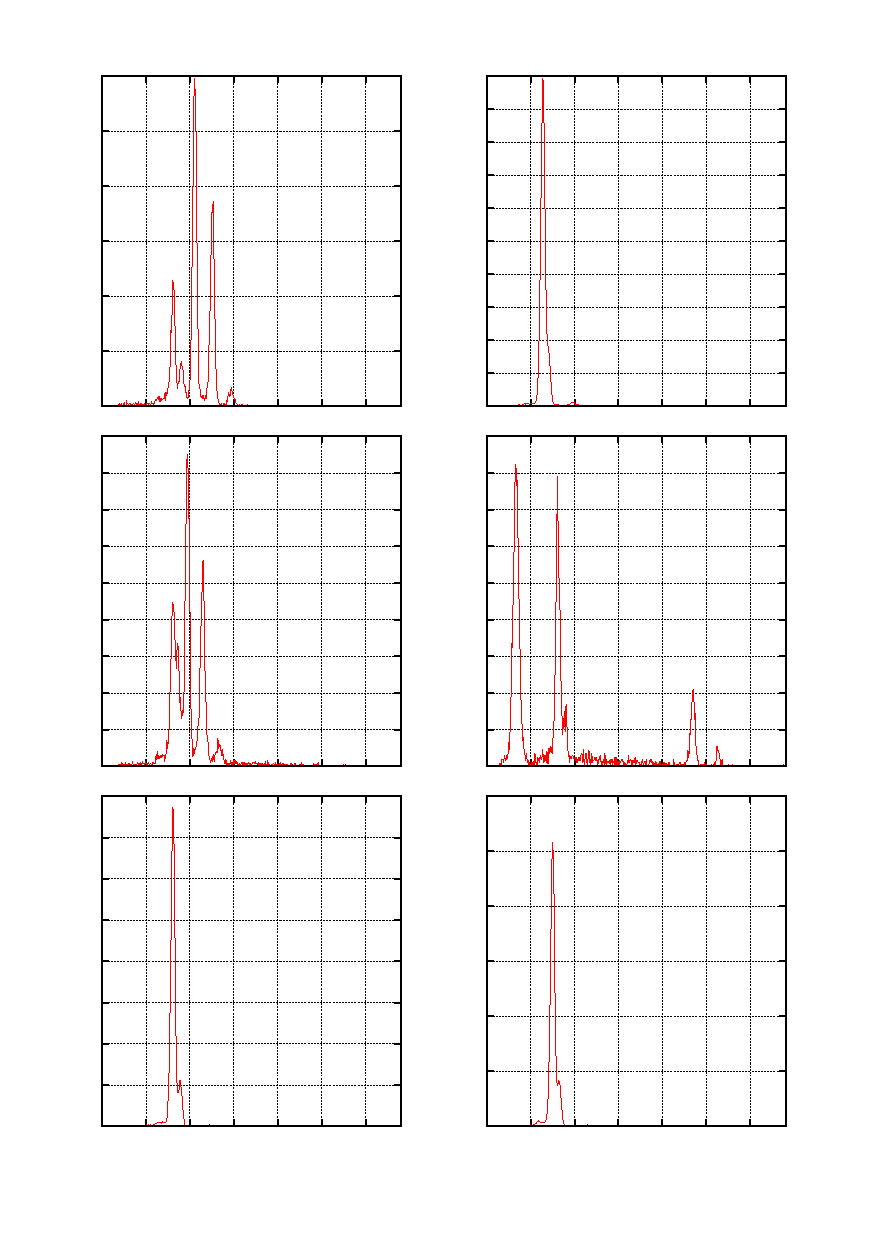
\includegraphics{./plots/referenzspektren1}}%
    \gplfronttext
  \end{picture}%
\endgroup

\end{figure}

\begin{figure}[h]
\centering
% GNUPLOT: LaTeX picture with Postscript
\begingroup
  \makeatletter
  \providecommand\color[2][]{%
    \GenericError{(gnuplot) \space\space\space\@spaces}{%
      Package color not loaded in conjunction with
      terminal option `colourtext'%
    }{See the gnuplot documentation for explanation.%
    }{Either use 'blacktext' in gnuplot or load the package
      color.sty in LaTeX.}%
    \renewcommand\color[2][]{}%
  }%
  \providecommand\includegraphics[2][]{%
    \GenericError{(gnuplot) \space\space\space\@spaces}{%
      Package graphicx or graphics not loaded%
    }{See the gnuplot documentation for explanation.%
    }{The gnuplot epslatex terminal needs graphicx.sty or graphics.sty.}%
    \renewcommand\includegraphics[2][]{}%
  }%
  \providecommand\rotatebox[2]{#2}%
  \@ifundefined{ifGPcolor}{%
    \newif\ifGPcolor
    \GPcolortrue
  }{}%
  \@ifundefined{ifGPblacktext}{%
    \newif\ifGPblacktext
    \GPblacktexttrue
  }{}%
  % define a \g@addto@macro without @ in the name:
  \let\gplgaddtomacro\g@addto@macro
  % define empty templates for all commands taking text:
  \gdef\gplbacktext{}%
  \gdef\gplfronttext{}%
  \makeatother
  \ifGPblacktext
    % no textcolor at all
    \def\colorrgb#1{}%
    \def\colorgray#1{}%
  \else
    % gray or color?
    \ifGPcolor
      \def\colorrgb#1{\color[rgb]{#1}}%
      \def\colorgray#1{\color[gray]{#1}}%
      \expandafter\def\csname LTw\endcsname{\color{white}}%
      \expandafter\def\csname LTb\endcsname{\color{black}}%
      \expandafter\def\csname LTa\endcsname{\color{black}}%
      \expandafter\def\csname LT0\endcsname{\color[rgb]{1,0,0}}%
      \expandafter\def\csname LT1\endcsname{\color[rgb]{0,1,0}}%
      \expandafter\def\csname LT2\endcsname{\color[rgb]{0,0,1}}%
      \expandafter\def\csname LT3\endcsname{\color[rgb]{1,0,1}}%
      \expandafter\def\csname LT4\endcsname{\color[rgb]{0,1,1}}%
      \expandafter\def\csname LT5\endcsname{\color[rgb]{1,1,0}}%
      \expandafter\def\csname LT6\endcsname{\color[rgb]{0,0,0}}%
      \expandafter\def\csname LT7\endcsname{\color[rgb]{1,0.3,0}}%
      \expandafter\def\csname LT8\endcsname{\color[rgb]{0.5,0.5,0.5}}%
    \else
      % gray
      \def\colorrgb#1{\color{black}}%
      \def\colorgray#1{\color[gray]{#1}}%
      \expandafter\def\csname LTw\endcsname{\color{white}}%
      \expandafter\def\csname LTb\endcsname{\color{black}}%
      \expandafter\def\csname LTa\endcsname{\color{black}}%
      \expandafter\def\csname LT0\endcsname{\color{black}}%
      \expandafter\def\csname LT1\endcsname{\color{black}}%
      \expandafter\def\csname LT2\endcsname{\color{black}}%
      \expandafter\def\csname LT3\endcsname{\color{black}}%
      \expandafter\def\csname LT4\endcsname{\color{black}}%
      \expandafter\def\csname LT5\endcsname{\color{black}}%
      \expandafter\def\csname LT6\endcsname{\color{black}}%
      \expandafter\def\csname LT7\endcsname{\color{black}}%
      \expandafter\def\csname LT8\endcsname{\color{black}}%
    \fi
  \fi
  \setlength{\unitlength}{0.0500bp}%
  \begin{picture}(8206.00,11520.00)%
      \csname LTb\endcsname%
      \put(4103,11300){\makebox(0,0){\strut{}Referenzspektren Teil 2}}%
    \gplgaddtomacro\gplbacktext{%
      \csname LTb\endcsname%
      \put(688,7776){\makebox(0,0)[r]{\strut{}0}}%
      \csname LTb\endcsname%
      \put(688,8409){\makebox(0,0)[r]{\strut{}20}}%
      \csname LTb\endcsname%
      \put(688,9043){\makebox(0,0)[r]{\strut{}40}}%
      \csname LTb\endcsname%
      \put(688,9676){\makebox(0,0)[r]{\strut{}60}}%
      \csname LTb\endcsname%
      \put(688,10310){\makebox(0,0)[r]{\strut{}80}}%
      \csname LTb\endcsname%
      \put(688,10943){\makebox(0,0)[r]{\strut{}100}}%
      \csname LTb\endcsname%
      \put(820,7556){\makebox(0,0){\strut{} 0}}%
      \csname LTb\endcsname%
      \put(1539,7556){\makebox(0,0){\strut{} 128}}%
      \csname LTb\endcsname%
      \put(2259,7556){\makebox(0,0){\strut{} 256}}%
      \csname LTb\endcsname%
      \put(2978,7556){\makebox(0,0){\strut{} 384}}%
      \put(50,9359){\rotatebox{-270}{\makebox(0,0){\strut{}Counts}}}%
      \put(3347,10690){\makebox(0,0)[l]{\strut{}Ag}}%
    }%
    \gplgaddtomacro\gplfronttext{%
    }%
    \gplgaddtomacro\gplbacktext{%
      \csname LTb\endcsname%
      \put(4381,7776){\makebox(0,0)[r]{\strut{}0}}%
      \csname LTb\endcsname%
      \put(4381,8172){\makebox(0,0)[r]{\strut{}500}}%
      \csname LTb\endcsname%
      \put(4381,8568){\makebox(0,0)[r]{\strut{}1000}}%
      \csname LTb\endcsname%
      \put(4381,8964){\makebox(0,0)[r]{\strut{}1500}}%
      \csname LTb\endcsname%
      \put(4381,9359){\makebox(0,0)[r]{\strut{}2000}}%
      \csname LTb\endcsname%
      \put(4381,9755){\makebox(0,0)[r]{\strut{}2500}}%
      \csname LTb\endcsname%
      \put(4381,10151){\makebox(0,0)[r]{\strut{}3000}}%
      \csname LTb\endcsname%
      \put(4381,10547){\makebox(0,0)[r]{\strut{}3500}}%
      \csname LTb\endcsname%
      \put(4381,10943){\makebox(0,0)[r]{\strut{}4000}}%
      \csname LTb\endcsname%
      \put(4513,7556){\makebox(0,0){\strut{} 0}}%
      \csname LTb\endcsname%
      \put(5232,7556){\makebox(0,0){\strut{} 128}}%
      \csname LTb\endcsname%
      \put(5951,7556){\makebox(0,0){\strut{} 256}}%
      \csname LTb\endcsname%
      \put(6670,7556){\makebox(0,0){\strut{} 384}}%
      \put(7039,10690){\makebox(0,0)[l]{\strut{}Ti}}%
    }%
    \gplgaddtomacro\gplfronttext{%
    }%
    \gplgaddtomacro\gplbacktext{%
      \csname LTb\endcsname%
      \put(688,4320){\makebox(0,0)[r]{\strut{}0}}%
      \csname LTb\endcsname%
      \put(688,4716){\makebox(0,0)[r]{\strut{}100}}%
      \csname LTb\endcsname%
      \put(688,5112){\makebox(0,0)[r]{\strut{}200}}%
      \csname LTb\endcsname%
      \put(688,5508){\makebox(0,0)[r]{\strut{}300}}%
      \csname LTb\endcsname%
      \put(688,5904){\makebox(0,0)[r]{\strut{}400}}%
      \csname LTb\endcsname%
      \put(688,6299){\makebox(0,0)[r]{\strut{}500}}%
      \csname LTb\endcsname%
      \put(688,6695){\makebox(0,0)[r]{\strut{}600}}%
      \csname LTb\endcsname%
      \put(688,7091){\makebox(0,0)[r]{\strut{}700}}%
      \csname LTb\endcsname%
      \put(688,7487){\makebox(0,0)[r]{\strut{}800}}%
      \csname LTb\endcsname%
      \put(820,4100){\makebox(0,0){\strut{} 0}}%
      \csname LTb\endcsname%
      \put(1539,4100){\makebox(0,0){\strut{} 128}}%
      \csname LTb\endcsname%
      \put(2259,4100){\makebox(0,0){\strut{} 256}}%
      \csname LTb\endcsname%
      \put(2978,4100){\makebox(0,0){\strut{} 384}}%
      \put(50,5903){\rotatebox{-270}{\makebox(0,0){\strut{}Counts}}}%
      \put(3347,7234){\makebox(0,0)[l]{\strut{}W}}%
    }%
    \gplgaddtomacro\gplfronttext{%
    }%
    \gplgaddtomacro\gplbacktext{%
      \csname LTb\endcsname%
      \put(4381,4320){\makebox(0,0)[r]{\strut{}0}}%
      \csname LTb\endcsname%
      \put(4381,4953){\makebox(0,0)[r]{\strut{}50}}%
      \csname LTb\endcsname%
      \put(4381,5587){\makebox(0,0)[r]{\strut{}100}}%
      \csname LTb\endcsname%
      \put(4381,6220){\makebox(0,0)[r]{\strut{}150}}%
      \csname LTb\endcsname%
      \put(4381,6854){\makebox(0,0)[r]{\strut{}200}}%
      \csname LTb\endcsname%
      \put(4381,7487){\makebox(0,0)[r]{\strut{}250}}%
      \csname LTb\endcsname%
      \put(4513,4100){\makebox(0,0){\strut{} 0}}%
      \csname LTb\endcsname%
      \put(5232,4100){\makebox(0,0){\strut{} 128}}%
      \csname LTb\endcsname%
      \put(5951,4100){\makebox(0,0){\strut{} 256}}%
      \csname LTb\endcsname%
      \put(6670,4100){\makebox(0,0){\strut{} 384}}%
      \put(7039,7234){\makebox(0,0)[l]{\strut{}Sn}}%
    }%
    \gplgaddtomacro\gplfronttext{%
    }%
    \gplgaddtomacro\gplbacktext{%
      \csname LTb\endcsname%
      \put(688,863){\makebox(0,0)[r]{\strut{}0}}%
      \csname LTb\endcsname%
      \put(688,1259){\makebox(0,0)[r]{\strut{}500}}%
      \csname LTb\endcsname%
      \put(688,1655){\makebox(0,0)[r]{\strut{}1000}}%
      \csname LTb\endcsname%
      \put(688,2051){\makebox(0,0)[r]{\strut{}1500}}%
      \csname LTb\endcsname%
      \put(688,2447){\makebox(0,0)[r]{\strut{}2000}}%
      \csname LTb\endcsname%
      \put(688,2843){\makebox(0,0)[r]{\strut{}2500}}%
      \csname LTb\endcsname%
      \put(688,3239){\makebox(0,0)[r]{\strut{}3000}}%
      \csname LTb\endcsname%
      \put(688,3635){\makebox(0,0)[r]{\strut{}3500}}%
      \csname LTb\endcsname%
      \put(688,4031){\makebox(0,0)[r]{\strut{}4000}}%
      \csname LTb\endcsname%
      \put(820,643){\makebox(0,0){\strut{} 0}}%
      \csname LTb\endcsname%
      \put(1539,643){\makebox(0,0){\strut{} 128}}%
      \csname LTb\endcsname%
      \put(2259,643){\makebox(0,0){\strut{} 256}}%
      \csname LTb\endcsname%
      \put(2978,643){\makebox(0,0){\strut{} 384}}%
      \put(-82,2447){\rotatebox{-270}{\makebox(0,0){\strut{}Counts}}}%
      \put(2256,313){\makebox(0,0){\strut{}Kanalnummer}}%
      \put(3347,3778){\makebox(0,0)[l]{\strut{}Zn}}%
    }%
    \gplgaddtomacro\gplfronttext{%
    }%
    \gplgaddtomacro\gplbacktext{%
      \csname LTb\endcsname%
      \put(4381,863){\makebox(0,0)[r]{\strut{}0}}%
      \csname LTb\endcsname%
      \put(4381,1259){\makebox(0,0)[r]{\strut{}100}}%
      \csname LTb\endcsname%
      \put(4381,1655){\makebox(0,0)[r]{\strut{}200}}%
      \csname LTb\endcsname%
      \put(4381,2051){\makebox(0,0)[r]{\strut{}300}}%
      \csname LTb\endcsname%
      \put(4381,2447){\makebox(0,0)[r]{\strut{}400}}%
      \csname LTb\endcsname%
      \put(4381,2843){\makebox(0,0)[r]{\strut{}500}}%
      \csname LTb\endcsname%
      \put(4381,3239){\makebox(0,0)[r]{\strut{}600}}%
      \csname LTb\endcsname%
      \put(4381,3635){\makebox(0,0)[r]{\strut{}700}}%
      \csname LTb\endcsname%
      \put(4381,4031){\makebox(0,0)[r]{\strut{}800}}%
      \csname LTb\endcsname%
      \put(4513,643){\makebox(0,0){\strut{} 0}}%
      \csname LTb\endcsname%
      \put(5232,643){\makebox(0,0){\strut{} 128}}%
      \csname LTb\endcsname%
      \put(5951,643){\makebox(0,0){\strut{} 256}}%
      \csname LTb\endcsname%
      \put(6670,643){\makebox(0,0){\strut{} 384}}%
      \put(5948,313){\makebox(0,0){\strut{}Kanalnummer}}%
      \put(7039,3778){\makebox(0,0)[l]{\strut{}Zr}}%
    }%
    \gplgaddtomacro\gplfronttext{%
    }%
    \gplbacktext
    \put(0,0){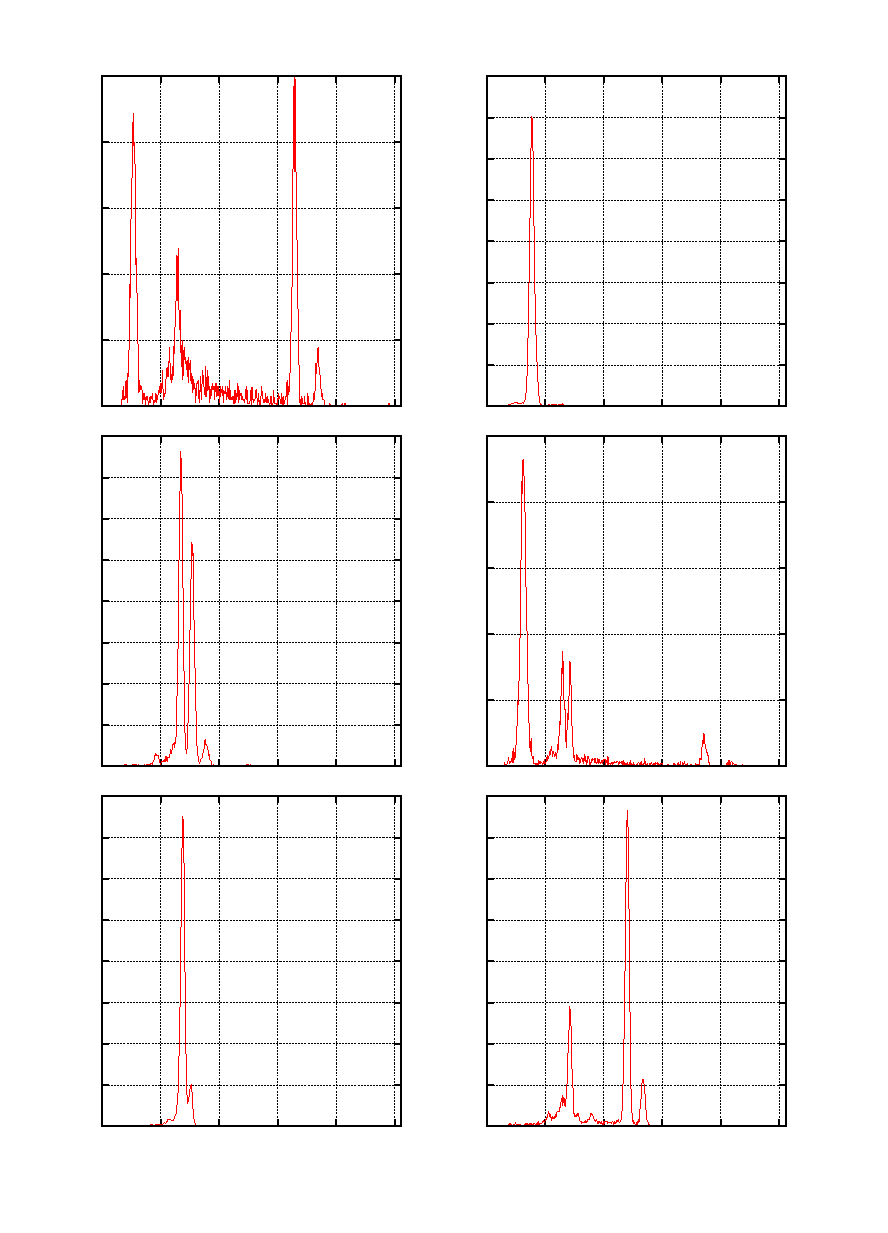
\includegraphics{./plots/referenzspektren2}}%
    \gplfronttext
  \end{picture}%
\endgroup

\end{figure}

\end{appendix}

\end{document}
